\documentclass[twoside]{book}

% Packages required by doxygen
\usepackage{fixltx2e}
\usepackage{calc}
\usepackage{doxygen}
\usepackage[export]{adjustbox} % also loads graphicx
\usepackage{graphicx}
\usepackage[utf8]{inputenc}
\usepackage{makeidx}
\usepackage{multicol}
\usepackage{multirow}
\PassOptionsToPackage{warn}{textcomp}
\usepackage{textcomp}
\usepackage[nointegrals]{wasysym}
\usepackage[table]{xcolor}

% Font selection
\usepackage[T1]{fontenc}
\usepackage[scaled=.90]{helvet}
\usepackage{courier}
\usepackage{amssymb}
\usepackage{sectsty}
\renewcommand{\familydefault}{\sfdefault}
\allsectionsfont{%
  \fontseries{bc}\selectfont%
  \color{darkgray}%
}
\renewcommand{\DoxyLabelFont}{%
  \fontseries{bc}\selectfont%
  \color{darkgray}%
}
\newcommand{\+}{\discretionary{\mbox{\scriptsize$\hookleftarrow$}}{}{}}

% Page & text layout
\usepackage{geometry}
\geometry{%
  a4paper,%
  top=2.5cm,%
  bottom=2.5cm,%
  left=2.5cm,%
  right=2.5cm%
}
\tolerance=750
\hfuzz=15pt
\hbadness=750
\setlength{\emergencystretch}{15pt}
\setlength{\parindent}{0cm}
\setlength{\parskip}{3ex plus 2ex minus 2ex}
\makeatletter
\renewcommand{\paragraph}{%
  \@startsection{paragraph}{4}{0ex}{-1.0ex}{1.0ex}{%
    \normalfont\normalsize\bfseries\SS@parafont%
  }%
}
\renewcommand{\subparagraph}{%
  \@startsection{subparagraph}{5}{0ex}{-1.0ex}{1.0ex}{%
    \normalfont\normalsize\bfseries\SS@subparafont%
  }%
}
\makeatother

% Headers & footers
\usepackage{fancyhdr}
\pagestyle{fancyplain}
\fancyhead[LE]{\fancyplain{}{\bfseries\thepage}}
\fancyhead[CE]{\fancyplain{}{}}
\fancyhead[RE]{\fancyplain{}{\bfseries\leftmark}}
\fancyhead[LO]{\fancyplain{}{\bfseries\rightmark}}
\fancyhead[CO]{\fancyplain{}{}}
\fancyhead[RO]{\fancyplain{}{\bfseries\thepage}}
\fancyfoot[LE]{\fancyplain{}{}}
\fancyfoot[CE]{\fancyplain{}{}}
\fancyfoot[RE]{\fancyplain{}{\bfseries\scriptsize Generated by Doxygen }}
\fancyfoot[LO]{\fancyplain{}{\bfseries\scriptsize Generated by Doxygen }}
\fancyfoot[CO]{\fancyplain{}{}}
\fancyfoot[RO]{\fancyplain{}{}}
\renewcommand{\footrulewidth}{0.4pt}
\renewcommand{\chaptermark}[1]{%
  \markboth{#1}{}%
}
\renewcommand{\sectionmark}[1]{%
  \markright{\thesection\ #1}%
}

% Indices & bibliography
\usepackage{natbib}
\usepackage[titles]{tocloft}
\setcounter{tocdepth}{3}
\setcounter{secnumdepth}{5}
\makeindex

% Hyperlinks (required, but should be loaded last)
\usepackage{ifpdf}
\ifpdf
  \usepackage[pdftex,pagebackref=true]{hyperref}
\else
  \usepackage[ps2pdf,pagebackref=true]{hyperref}
\fi
\hypersetup{%
  colorlinks=true,%
  linkcolor=blue,%
  citecolor=blue,%
  unicode%
}

% Custom commands
\newcommand{\clearemptydoublepage}{%
  \newpage{\pagestyle{empty}\cleardoublepage}%
}

\usepackage{caption}
\captionsetup{labelsep=space,justification=centering,font={bf},singlelinecheck=off,skip=4pt,position=top}

%===== C O N T E N T S =====

\begin{document}

% Titlepage & ToC
\hypersetup{pageanchor=false,
             bookmarksnumbered=true,
             pdfencoding=unicode
            }
\pagenumbering{alph}
\begin{titlepage}
\vspace*{7cm}
\begin{center}%
{\Large Ascii-\/\+Crawler }\\
\vspace*{1cm}
{\large Generated by Doxygen 1.8.13}\\
\end{center}
\end{titlepage}
\clearemptydoublepage
\pagenumbering{roman}
\tableofcontents
\clearemptydoublepage
\pagenumbering{arabic}
\hypersetup{pageanchor=true}

%--- Begin generated contents ---
\chapter{Ascii-\/\+Crawler}
\label{index}\hypertarget{index}{}This is a student project for the course \char`\"{}technical documentation\char`\"{} at the University Bremen.

Participants\+: \tabulinesep=1mm
\begin{longtabu} spread 0pt [c]{*{2}{|X[-1]}|}
\hline
\rowcolor{\tableheadbgcolor}\textbf{ name }&\textbf{ matriculation number  }\\\cline{1-2}
\endfirsthead
\hline
\endfoot
\hline
\rowcolor{\tableheadbgcolor}\textbf{ name }&\textbf{ matriculation number  }\\\cline{1-2}
\endhead
Leon Hansen &3066551 \\\cline{1-2}
Felix Schmidt &3115378 \\\cline{1-2}
\end{longtabu}

\chapter{Hierarchical Index}
\section{Class Hierarchy}
This inheritance list is sorted roughly, but not completely, alphabetically\+:\begin{DoxyCompactList}
\item \contentsline{section}{asciicrawler.\+Board}{\pageref{classasciicrawler_1_1Board}}{}
\item \contentsline{section}{asciicrawler.\+Board\+Object}{\pageref{classasciicrawler_1_1BoardObject}}{}
\begin{DoxyCompactList}
\item \contentsline{section}{asciicrawler.\+Air}{\pageref{classasciicrawler_1_1Air}}{}
\item \contentsline{section}{asciicrawler.\+Exit}{\pageref{classasciicrawler_1_1Exit}}{}
\item \contentsline{section}{asciicrawler.\+Gold}{\pageref{classasciicrawler_1_1Gold}}{}
\item \contentsline{section}{asciicrawler.\+Mob}{\pageref{classasciicrawler_1_1Mob}}{}
\begin{DoxyCompactList}
\item \contentsline{section}{asciicrawler.\+Enemy}{\pageref{classasciicrawler_1_1Enemy}}{}
\item \contentsline{section}{asciicrawler.\+Player}{\pageref{classasciicrawler_1_1Player}}{}
\end{DoxyCompactList}
\item \contentsline{section}{asciicrawler.\+Wall}{\pageref{classasciicrawler_1_1Wall}}{}
\item \contentsline{section}{asciicrawler.\+Water}{\pageref{classasciicrawler_1_1Water}}{}
\end{DoxyCompactList}
\item \contentsline{section}{asciicrawler.\+Direction}{\pageref{enumasciicrawler_1_1Direction}}{}
\item \contentsline{section}{asciicrawler.\+Game}{\pageref{classasciicrawler_1_1Game}}{}
\item \contentsline{section}{asciicrawler.\+Key\+Manager}{\pageref{classasciicrawler_1_1KeyManager}}{}
\item \contentsline{section}{Main}{\pageref{classMain}}{}
\item Frame\begin{DoxyCompactList}
\item \contentsline{section}{asciicrawler.\+Display}{\pageref{classasciicrawler_1_1Display}}{}
\end{DoxyCompactList}
\item Timer\+Task\begin{DoxyCompactList}
\item \contentsline{section}{asciicrawler.\+Game\+Ticker}{\pageref{classasciicrawler_1_1GameTicker}}{}
\end{DoxyCompactList}
\end{DoxyCompactList}

\chapter{Class Index}
\section{Class List}
Here are the classes, structs, unions and interfaces with brief descriptions\+:\begin{DoxyCompactList}
\item\contentsline{section}{\hyperlink{classasciicrawler_1_1Air}{asciicrawler.\+Air} \\*\hyperlink{classasciicrawler_1_1Air}{Air} is a board object. On this fields of the board the player and the enemys are walking along the dungeon }{\pageref{classasciicrawler_1_1Air}}{}
\item\contentsline{section}{\hyperlink{classasciicrawler_1_1Board}{asciicrawler.\+Board} \\*\hyperlink{classasciicrawler_1_1Board}{Board} stores all configurations of the current dungeon }{\pageref{classasciicrawler_1_1Board}}{}
\item\contentsline{section}{\hyperlink{classasciicrawler_1_1BoardObject}{asciicrawler.\+Board\+Object} \\*Is the abstract class of several board objects }{\pageref{classasciicrawler_1_1BoardObject}}{}
\item\contentsline{section}{\hyperlink{enumasciicrawler_1_1Direction}{asciicrawler.\+Direction} \\*This enum defines all walking directions of the mobs }{\pageref{enumasciicrawler_1_1Direction}}{}
\item\contentsline{section}{\hyperlink{classasciicrawler_1_1Display}{asciicrawler.\+Display} \\*Class is the display of the game and handles the rendering }{\pageref{classasciicrawler_1_1Display}}{}
\item\contentsline{section}{\hyperlink{classasciicrawler_1_1Enemy}{asciicrawler.\+Enemy} \\*Contains the \hyperlink{classasciicrawler_1_1Enemy}{Enemy} AI }{\pageref{classasciicrawler_1_1Enemy}}{}
\item\contentsline{section}{\hyperlink{classasciicrawler_1_1Exit}{asciicrawler.\+Exit} \\*\hyperlink{classasciicrawler_1_1Exit}{Exit} is a board object. It is the field in the game where the player starts and the ends the level }{\pageref{classasciicrawler_1_1Exit}}{}
\item\contentsline{section}{\hyperlink{classasciicrawler_1_1Game}{asciicrawler.\+Game} }{\pageref{classasciicrawler_1_1Game}}{}
\item\contentsline{section}{\hyperlink{classasciicrawler_1_1GameTicker}{asciicrawler.\+Game\+Ticker} \\*This will handle all game ticks and the movement of player/enemy }{\pageref{classasciicrawler_1_1GameTicker}}{}
\item\contentsline{section}{\hyperlink{classasciicrawler_1_1Gold}{asciicrawler.\+Gold} \\*\hyperlink{classasciicrawler_1_1Gold}{Gold} is a board object. The \hyperlink{classasciicrawler_1_1Player}{Player} have to reach this field one time and then he can go back to the Exit-\/field }{\pageref{classasciicrawler_1_1Gold}}{}
\item\contentsline{section}{\hyperlink{classasciicrawler_1_1KeyManager}{asciicrawler.\+Key\+Manager} \\*Mangaer to assign actions to specific key events }{\pageref{classasciicrawler_1_1KeyManager}}{}
\item\contentsline{section}{\hyperlink{classMain}{Main} }{\pageref{classMain}}{}
\item\contentsline{section}{\hyperlink{classasciicrawler_1_1Mob}{asciicrawler.\+Mob} \\*Is the abstract class of several mob objects }{\pageref{classasciicrawler_1_1Mob}}{}
\item\contentsline{section}{\hyperlink{classasciicrawler_1_1Player}{asciicrawler.\+Player} \\*\hyperlink{classasciicrawler_1_1Player}{Player} is class derived from mob. It specifices the abilities and and actions of a player }{\pageref{classasciicrawler_1_1Player}}{}
\item\contentsline{section}{\hyperlink{classasciicrawler_1_1Wall}{asciicrawler.\+Wall} \\*\hyperlink{classasciicrawler_1_1Wall}{Wall} is a board object. This field can not entered by any mob }{\pageref{classasciicrawler_1_1Wall}}{}
\item\contentsline{section}{\hyperlink{classasciicrawler_1_1Water}{asciicrawler.\+Water} \\*\hyperlink{classasciicrawler_1_1Water}{Water} is a board object. This field can not entered by any mob }{\pageref{classasciicrawler_1_1Water}}{}
\end{DoxyCompactList}

\chapter{Class Documentation}
\hypertarget{classasciicrawler_1_1Air}{}\section{asciicrawler.\+Air Class Reference}
\label{classasciicrawler_1_1Air}\index{asciicrawler.\+Air@{asciicrawler.\+Air}}


\hyperlink{classasciicrawler_1_1Air}{Air} is a board object. On this fields of the board the player and the enemys are walking along the dungeon.  


Inheritance diagram for asciicrawler.\+Air\+:\begin{figure}[H]
\begin{center}
\leavevmode
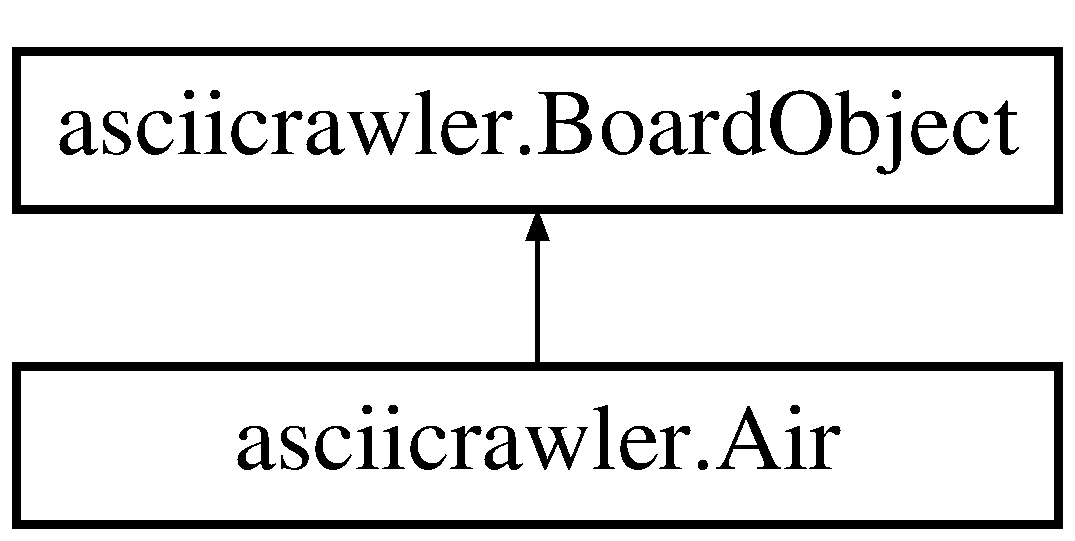
\includegraphics[height=2.000000cm]{classasciicrawler_1_1Air}
\end{center}
\end{figure}
\subsection*{Public Member Functions}
\begin{DoxyCompactItemize}
\item 
boolean \hyperlink{classasciicrawler_1_1Air_ac674c1f8c90cdda29eb7f12ed794eb4c}{can\+Enter} ()
\item 
Color \hyperlink{classasciicrawler_1_1Air_a4f2f155658f758d97a85944b117a87f3}{get\+Color} ()
\end{DoxyCompactItemize}


\subsection{Detailed Description}
\hyperlink{classasciicrawler_1_1Air}{Air} is a board object. On this fields of the board the player and the enemys are walking along the dungeon. 

\begin{DoxyAuthor}{Author}
Leon Hansen, Felix Schmidt 
\end{DoxyAuthor}
\begin{DoxyVersion}{Version}
1.\+0 
\end{DoxyVersion}


\subsection{Member Function Documentation}
\mbox{\Hypertarget{classasciicrawler_1_1Air_ac674c1f8c90cdda29eb7f12ed794eb4c}\label{classasciicrawler_1_1Air_ac674c1f8c90cdda29eb7f12ed794eb4c}} 
\index{asciicrawler\+::\+Air@{asciicrawler\+::\+Air}!can\+Enter@{can\+Enter}}
\index{can\+Enter@{can\+Enter}!asciicrawler\+::\+Air@{asciicrawler\+::\+Air}}
\subsubsection{\texorpdfstring{can\+Enter()}{canEnter()}}
{\footnotesize\ttfamily boolean asciicrawler.\+Air.\+can\+Enter (\begin{DoxyParamCaption}{ }\end{DoxyParamCaption})\hspace{0.3cm}{\ttfamily [inline]}}

Checks if the \hyperlink{classasciicrawler_1_1Mob}{Mob} can access this type of field \mbox{\Hypertarget{classasciicrawler_1_1Air_a4f2f155658f758d97a85944b117a87f3}\label{classasciicrawler_1_1Air_a4f2f155658f758d97a85944b117a87f3}} 
\index{asciicrawler\+::\+Air@{asciicrawler\+::\+Air}!get\+Color@{get\+Color}}
\index{get\+Color@{get\+Color}!asciicrawler\+::\+Air@{asciicrawler\+::\+Air}}
\subsubsection{\texorpdfstring{get\+Color()}{getColor()}}
{\footnotesize\ttfamily Color asciicrawler.\+Air.\+get\+Color (\begin{DoxyParamCaption}{ }\end{DoxyParamCaption})\hspace{0.3cm}{\ttfamily [inline]}}

Returns the Color of the field 

The documentation for this class was generated from the following file\+:\begin{DoxyCompactItemize}
\item 
/home/felix/\+Documents/\+Uni/\+Master/1. Semester/\+Technische Dokumentation/\+Spiel/\+Ascii-\/\+Crawler/src/asciicrawler/Air.\+java\end{DoxyCompactItemize}

\hypertarget{classasciicrawler_1_1Board}{}\section{asciicrawler.\+Board Class Reference}
\label{classasciicrawler_1_1Board}\index{asciicrawler.\+Board@{asciicrawler.\+Board}}
\subsection*{Public Member Functions}
\begin{DoxyCompactItemize}
\item 
\mbox{\Hypertarget{classasciicrawler_1_1Board_aa6d40676bda8efa863277524168d575d}\label{classasciicrawler_1_1Board_aa6d40676bda8efa863277524168d575d}} 
void {\bfseries reset} ()
\item 
\mbox{\Hypertarget{classasciicrawler_1_1Board_ab1cf721c223fcdafc141fe858c243d60}\label{classasciicrawler_1_1Board_ab1cf721c223fcdafc141fe858c243d60}} 
void {\bfseries set\+Board\+Object} (int x, int y, \hyperlink{classasciicrawler_1_1BoardObject}{Board\+Object} Item)
\item 
\mbox{\Hypertarget{classasciicrawler_1_1Board_a059f9044f0d0f6dc9c5729c9c8c082a2}\label{classasciicrawler_1_1Board_a059f9044f0d0f6dc9c5729c9c8c082a2}} 
\hyperlink{classasciicrawler_1_1BoardObject}{Board\+Object} {\bfseries get\+Board\+Object} (int x, int y)
\item 
\mbox{\Hypertarget{classasciicrawler_1_1Board_af8fabfec19cd00bb4205e656c505789f}\label{classasciicrawler_1_1Board_af8fabfec19cd00bb4205e656c505789f}} 
void {\bfseries generate\+Dungeon} ()
\end{DoxyCompactItemize}
\subsection*{Static Public Member Functions}
\begin{DoxyCompactItemize}
\item 
\mbox{\Hypertarget{classasciicrawler_1_1Board_abf113bdc50898a0f64eb3611b98111ea}\label{classasciicrawler_1_1Board_abf113bdc50898a0f64eb3611b98111ea}} 
static boolean {\bfseries is\+On\+Board} (int x, int y)
\item 
\mbox{\Hypertarget{classasciicrawler_1_1Board_a3ec369e192af66b0aa62f0a5ed5f18b0}\label{classasciicrawler_1_1Board_a3ec369e192af66b0aa62f0a5ed5f18b0}} 
static int {\bfseries get\+X\+Offset} (\hyperlink{enumasciicrawler_1_1Direction}{Direction} d)
\item 
\mbox{\Hypertarget{classasciicrawler_1_1Board_a8de1ca8752186e89183ec33c24316c41}\label{classasciicrawler_1_1Board_a8de1ca8752186e89183ec33c24316c41}} 
static int {\bfseries get\+Y\+Offset} (\hyperlink{enumasciicrawler_1_1Direction}{Direction} d)
\item 
\mbox{\Hypertarget{classasciicrawler_1_1Board_a115e44d78ee7c3edbd83dba743433634}\label{classasciicrawler_1_1Board_a115e44d78ee7c3edbd83dba743433634}} 
static \hyperlink{enumasciicrawler_1_1Direction}{Direction} {\bfseries get\+Opposite} (\hyperlink{enumasciicrawler_1_1Direction}{Direction} d)
\end{DoxyCompactItemize}
\subsection*{Public Attributes}
\begin{DoxyCompactItemize}
\item 
\mbox{\Hypertarget{classasciicrawler_1_1Board_a1417cc9364dcde96656344cd1fbba64b}\label{classasciicrawler_1_1Board_a1417cc9364dcde96656344cd1fbba64b}} 
\hyperlink{classasciicrawler_1_1BoardObject}{Board\+Object} {\bfseries board\+Objects} \mbox{[}$\,$\mbox{]}\mbox{[}$\,$\mbox{]}
\end{DoxyCompactItemize}
\subsection*{Static Public Attributes}
\begin{DoxyCompactItemize}
\item 
\mbox{\Hypertarget{classasciicrawler_1_1Board_ab6f1d7d36e8e04c8208ed058db244034}\label{classasciicrawler_1_1Board_ab6f1d7d36e8e04c8208ed058db244034}} 
static final int {\bfseries width} = 30
\item 
\mbox{\Hypertarget{classasciicrawler_1_1Board_ae8172665a1917d5d6f4805233f90eef7}\label{classasciicrawler_1_1Board_ae8172665a1917d5d6f4805233f90eef7}} 
static final int {\bfseries height} = 20
\item 
\mbox{\Hypertarget{classasciicrawler_1_1Board_a762e31d070af0a6449676051bcf84792}\label{classasciicrawler_1_1Board_a762e31d070af0a6449676051bcf84792}} 
static final int {\bfseries number\+Of\+Enemies} = 5
\item 
\mbox{\Hypertarget{classasciicrawler_1_1Board_aecf0ad63bd90427ea239d3f4febb0daa}\label{classasciicrawler_1_1Board_aecf0ad63bd90427ea239d3f4febb0daa}} 
static final double {\bfseries water\+Chance} = 0.\+02
\item 
\mbox{\Hypertarget{classasciicrawler_1_1Board_ad8831627475937561ddc52c70fd93fa7}\label{classasciicrawler_1_1Board_ad8831627475937561ddc52c70fd93fa7}} 
static final \hyperlink{classasciicrawler_1_1Wall}{Wall} {\bfseries wall} = new \hyperlink{classasciicrawler_1_1Wall}{Wall}()
\item 
\mbox{\Hypertarget{classasciicrawler_1_1Board_affa435afb88723f5d8d1a25440c893a3}\label{classasciicrawler_1_1Board_affa435afb88723f5d8d1a25440c893a3}} 
static final \hyperlink{classasciicrawler_1_1Air}{Air} {\bfseries air} = new \hyperlink{classasciicrawler_1_1Air}{Air}()
\item 
\mbox{\Hypertarget{classasciicrawler_1_1Board_ad0b6ed4f52b14c790915eca84b0d42b0}\label{classasciicrawler_1_1Board_ad0b6ed4f52b14c790915eca84b0d42b0}} 
static final \hyperlink{classasciicrawler_1_1Water}{Water} {\bfseries water} = new \hyperlink{classasciicrawler_1_1Water}{Water}()
\item 
\mbox{\Hypertarget{classasciicrawler_1_1Board_af821e453812eaf8572780a71dacd23ce}\label{classasciicrawler_1_1Board_af821e453812eaf8572780a71dacd23ce}} 
static final \hyperlink{classasciicrawler_1_1Gold}{Gold} {\bfseries gold} = new \hyperlink{classasciicrawler_1_1Gold}{Gold}()
\item 
\mbox{\Hypertarget{classasciicrawler_1_1Board_a1b5144ca3bd142ab5545a67fa4cd2612}\label{classasciicrawler_1_1Board_a1b5144ca3bd142ab5545a67fa4cd2612}} 
static final \hyperlink{classasciicrawler_1_1Exit}{Exit} {\bfseries exit} = new \hyperlink{classasciicrawler_1_1Exit}{Exit}()
\item 
\mbox{\Hypertarget{classasciicrawler_1_1Board_aa15d853590a296fa341b734b21e79b43}\label{classasciicrawler_1_1Board_aa15d853590a296fa341b734b21e79b43}} 
static \hyperlink{classasciicrawler_1_1Enemy}{Enemy} \mbox{[}$\,$\mbox{]} {\bfseries enemies}
\item 
\mbox{\Hypertarget{classasciicrawler_1_1Board_ab6a0f4e30f00268e4b33473efedb1c83}\label{classasciicrawler_1_1Board_ab6a0f4e30f00268e4b33473efedb1c83}} 
static final \hyperlink{classasciicrawler_1_1Player}{Player} {\bfseries player} = new \hyperlink{classasciicrawler_1_1Player}{Player}()
\item 
static final List$<$ \hyperlink{enumasciicrawler_1_1Direction}{Direction} $>$ {\bfseries directions}
\end{DoxyCompactItemize}


\subsection{Detailed Description}
\hyperlink{classasciicrawler_1_1Board}{Board} stores all configurations of the current room

\begin{DoxyAuthor}{Author}
Leon Hansen, Felix Schmidt 
\end{DoxyAuthor}
\begin{DoxyVersion}{Version}
1.\+0 
\end{DoxyVersion}


\subsection{Member Data Documentation}
\mbox{\Hypertarget{classasciicrawler_1_1Board_a26b7ed317b5b9b2c8dd122a1cb369841}\label{classasciicrawler_1_1Board_a26b7ed317b5b9b2c8dd122a1cb369841}} 
\index{asciicrawler\+::\+Board@{asciicrawler\+::\+Board}!directions@{directions}}
\index{directions@{directions}!asciicrawler\+::\+Board@{asciicrawler\+::\+Board}}
\subsubsection{\texorpdfstring{directions}{directions}}
{\footnotesize\ttfamily final List$<$\hyperlink{enumasciicrawler_1_1Direction}{Direction}$>$ asciicrawler.\+Board.\+directions\hspace{0.3cm}{\ttfamily [static]}}

{\bfseries Initial value\+:}
\begin{DoxyCode}
= Arrays.asList(
            Direction.UP, Direction.RIGHT, Direction.DOWN, Direction.LEFT)
\end{DoxyCode}


The documentation for this class was generated from the following file\+:\begin{DoxyCompactItemize}
\item 
/home/felix/\+Documents/\+Uni/\+Master/1. Semester/\+Technische Dokumentation/\+Spiel/\+Ascii-\/\+Crawler/src/asciicrawler/Board.\+java\end{DoxyCompactItemize}

\hypertarget{classasciicrawler_1_1BoardObject}{}\section{asciicrawler.\+Board\+Object Class Reference}
\label{classasciicrawler_1_1BoardObject}\index{asciicrawler.\+Board\+Object@{asciicrawler.\+Board\+Object}}


Is the abstract class of several board objects.  


Inheritance diagram for asciicrawler.\+Board\+Object\+:\begin{figure}[H]
\begin{center}
\leavevmode
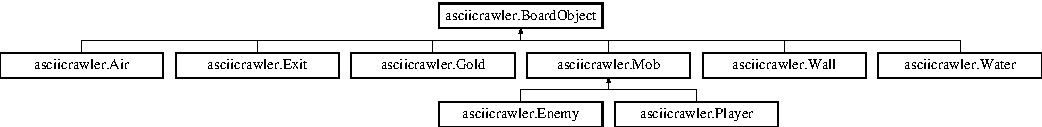
\includegraphics[height=1.707317cm]{classasciicrawler_1_1BoardObject}
\end{center}
\end{figure}
\subsection*{Public Member Functions}
\begin{DoxyCompactItemize}
\item 
abstract boolean \hyperlink{classasciicrawler_1_1BoardObject_a15efd8cf373a6cc12ca9b799a9fdc920}{can\+Enter} ()
\item 
abstract Color \hyperlink{classasciicrawler_1_1BoardObject_a64d367ca58baa54f85c5d266c0d01ca9}{get\+Color} ()
\item 
void \hyperlink{classasciicrawler_1_1BoardObject_aa9f18f80f01310da87221b78cf15de66}{On\+Enter} ()
\end{DoxyCompactItemize}


\subsection{Detailed Description}
Is the abstract class of several board objects. 

\begin{DoxyAuthor}{Author}
Leon Hansen, Felix Schmidt 
\end{DoxyAuthor}
\begin{DoxyVersion}{Version}
1.\+0 
\end{DoxyVersion}


\subsection{Member Function Documentation}
\mbox{\Hypertarget{classasciicrawler_1_1BoardObject_a15efd8cf373a6cc12ca9b799a9fdc920}\label{classasciicrawler_1_1BoardObject_a15efd8cf373a6cc12ca9b799a9fdc920}} 
\index{asciicrawler\+::\+Board\+Object@{asciicrawler\+::\+Board\+Object}!can\+Enter@{can\+Enter}}
\index{can\+Enter@{can\+Enter}!asciicrawler\+::\+Board\+Object@{asciicrawler\+::\+Board\+Object}}
\subsubsection{\texorpdfstring{can\+Enter()}{canEnter()}}
{\footnotesize\ttfamily abstract boolean asciicrawler.\+Board\+Object.\+can\+Enter (\begin{DoxyParamCaption}{ }\end{DoxyParamCaption})\hspace{0.3cm}{\ttfamily [abstract]}}

abstract method to check if a mob can enter the field \mbox{\Hypertarget{classasciicrawler_1_1BoardObject_a64d367ca58baa54f85c5d266c0d01ca9}\label{classasciicrawler_1_1BoardObject_a64d367ca58baa54f85c5d266c0d01ca9}} 
\index{asciicrawler\+::\+Board\+Object@{asciicrawler\+::\+Board\+Object}!get\+Color@{get\+Color}}
\index{get\+Color@{get\+Color}!asciicrawler\+::\+Board\+Object@{asciicrawler\+::\+Board\+Object}}
\subsubsection{\texorpdfstring{get\+Color()}{getColor()}}
{\footnotesize\ttfamily abstract Color asciicrawler.\+Board\+Object.\+get\+Color (\begin{DoxyParamCaption}{ }\end{DoxyParamCaption})\hspace{0.3cm}{\ttfamily [abstract]}}

abstract method to get the color of the field \mbox{\Hypertarget{classasciicrawler_1_1BoardObject_aa9f18f80f01310da87221b78cf15de66}\label{classasciicrawler_1_1BoardObject_aa9f18f80f01310da87221b78cf15de66}} 
\index{asciicrawler\+::\+Board\+Object@{asciicrawler\+::\+Board\+Object}!On\+Enter@{On\+Enter}}
\index{On\+Enter@{On\+Enter}!asciicrawler\+::\+Board\+Object@{asciicrawler\+::\+Board\+Object}}
\subsubsection{\texorpdfstring{On\+Enter()}{OnEnter()}}
{\footnotesize\ttfamily void asciicrawler.\+Board\+Object.\+On\+Enter (\begin{DoxyParamCaption}{ }\end{DoxyParamCaption})\hspace{0.3cm}{\ttfamily [inline]}}

abstract method to define what happens if a mob enter the field 

The documentation for this class was generated from the following file\+:\begin{DoxyCompactItemize}
\item 
/home/felix/\+Documents/\+Uni/\+Master/1. Semester/\+Technische Dokumentation/\+Spiel/\+Ascii-\/\+Crawler/src/asciicrawler/Board\+Object.\+java\end{DoxyCompactItemize}

\hypertarget{enumasciicrawler_1_1Direction}{}\section{asciicrawler.\+Direction Enum Reference}
\label{enumasciicrawler_1_1Direction}\index{asciicrawler.\+Direction@{asciicrawler.\+Direction}}


This enum defines all walking directions of the mobs.  


\subsection*{Public Attributes}
\begin{DoxyCompactItemize}
\item 
\hyperlink{enumasciicrawler_1_1Direction_a78902531c0af93fb05af7223491a4a1f}{S\+T\+AY}
\item 
\hyperlink{enumasciicrawler_1_1Direction_a6ddc24b03c5e790038cb48cf48ed8bb0}{UP}
\item 
\hyperlink{enumasciicrawler_1_1Direction_a90041664b85b23fec81f4cc7c5727382}{D\+O\+WN}
\item 
\hyperlink{enumasciicrawler_1_1Direction_a5bf2dba07f51db27f05c357baf2e1ff1}{L\+E\+FT}
\item 
\hyperlink{enumasciicrawler_1_1Direction_a2d6a7c41a905e8eda907cd59e9c80a55}{R\+I\+G\+HT}
\end{DoxyCompactItemize}


\subsection{Detailed Description}
This enum defines all walking directions of the mobs. 

\begin{DoxyAuthor}{Author}
Leon Hansen, Felix Schmidt 
\end{DoxyAuthor}
\begin{DoxyVersion}{Version}
1.\+0 
\end{DoxyVersion}


\subsection{Member Data Documentation}
\mbox{\Hypertarget{enumasciicrawler_1_1Direction_a90041664b85b23fec81f4cc7c5727382}\label{enumasciicrawler_1_1Direction_a90041664b85b23fec81f4cc7c5727382}} 
\index{asciicrawler\+::\+Direction@{asciicrawler\+::\+Direction}!D\+O\+WN@{D\+O\+WN}}
\index{D\+O\+WN@{D\+O\+WN}!asciicrawler\+::\+Direction@{asciicrawler\+::\+Direction}}
\subsubsection{\texorpdfstring{D\+O\+WN}{DOWN}}
{\footnotesize\ttfamily asciicrawler.\+Direction.\+D\+O\+WN}

state mob move down \mbox{\Hypertarget{enumasciicrawler_1_1Direction_a5bf2dba07f51db27f05c357baf2e1ff1}\label{enumasciicrawler_1_1Direction_a5bf2dba07f51db27f05c357baf2e1ff1}} 
\index{asciicrawler\+::\+Direction@{asciicrawler\+::\+Direction}!L\+E\+FT@{L\+E\+FT}}
\index{L\+E\+FT@{L\+E\+FT}!asciicrawler\+::\+Direction@{asciicrawler\+::\+Direction}}
\subsubsection{\texorpdfstring{L\+E\+FT}{LEFT}}
{\footnotesize\ttfamily asciicrawler.\+Direction.\+L\+E\+FT}

state mob move left \mbox{\Hypertarget{enumasciicrawler_1_1Direction_a2d6a7c41a905e8eda907cd59e9c80a55}\label{enumasciicrawler_1_1Direction_a2d6a7c41a905e8eda907cd59e9c80a55}} 
\index{asciicrawler\+::\+Direction@{asciicrawler\+::\+Direction}!R\+I\+G\+HT@{R\+I\+G\+HT}}
\index{R\+I\+G\+HT@{R\+I\+G\+HT}!asciicrawler\+::\+Direction@{asciicrawler\+::\+Direction}}
\subsubsection{\texorpdfstring{R\+I\+G\+HT}{RIGHT}}
{\footnotesize\ttfamily asciicrawler.\+Direction.\+R\+I\+G\+HT}

state mob move right \mbox{\Hypertarget{enumasciicrawler_1_1Direction_a78902531c0af93fb05af7223491a4a1f}\label{enumasciicrawler_1_1Direction_a78902531c0af93fb05af7223491a4a1f}} 
\index{asciicrawler\+::\+Direction@{asciicrawler\+::\+Direction}!S\+T\+AY@{S\+T\+AY}}
\index{S\+T\+AY@{S\+T\+AY}!asciicrawler\+::\+Direction@{asciicrawler\+::\+Direction}}
\subsubsection{\texorpdfstring{S\+T\+AY}{STAY}}
{\footnotesize\ttfamily asciicrawler.\+Direction.\+S\+T\+AY}

state mob doesn\textquotesingle{}t move \mbox{\Hypertarget{enumasciicrawler_1_1Direction_a6ddc24b03c5e790038cb48cf48ed8bb0}\label{enumasciicrawler_1_1Direction_a6ddc24b03c5e790038cb48cf48ed8bb0}} 
\index{asciicrawler\+::\+Direction@{asciicrawler\+::\+Direction}!UP@{UP}}
\index{UP@{UP}!asciicrawler\+::\+Direction@{asciicrawler\+::\+Direction}}
\subsubsection{\texorpdfstring{UP}{UP}}
{\footnotesize\ttfamily asciicrawler.\+Direction.\+UP}

state mob move up 

The documentation for this enum was generated from the following file\+:\begin{DoxyCompactItemize}
\item 
/home/felix/\+Documents/\+Uni/\+Master/1. Semester/\+Technische Dokumentation/\+Spiel/\+Ascii-\/\+Crawler/src/asciicrawler/Direction.\+java\end{DoxyCompactItemize}

\hypertarget{classasciicrawler_1_1Display}{}\section{asciicrawler.\+Display Class Reference}
\label{classasciicrawler_1_1Display}\index{asciicrawler.\+Display@{asciicrawler.\+Display}}


Class is the display of the game and handles the rendering.  


Inheritance diagram for asciicrawler.\+Display\+:\begin{figure}[H]
\begin{center}
\leavevmode
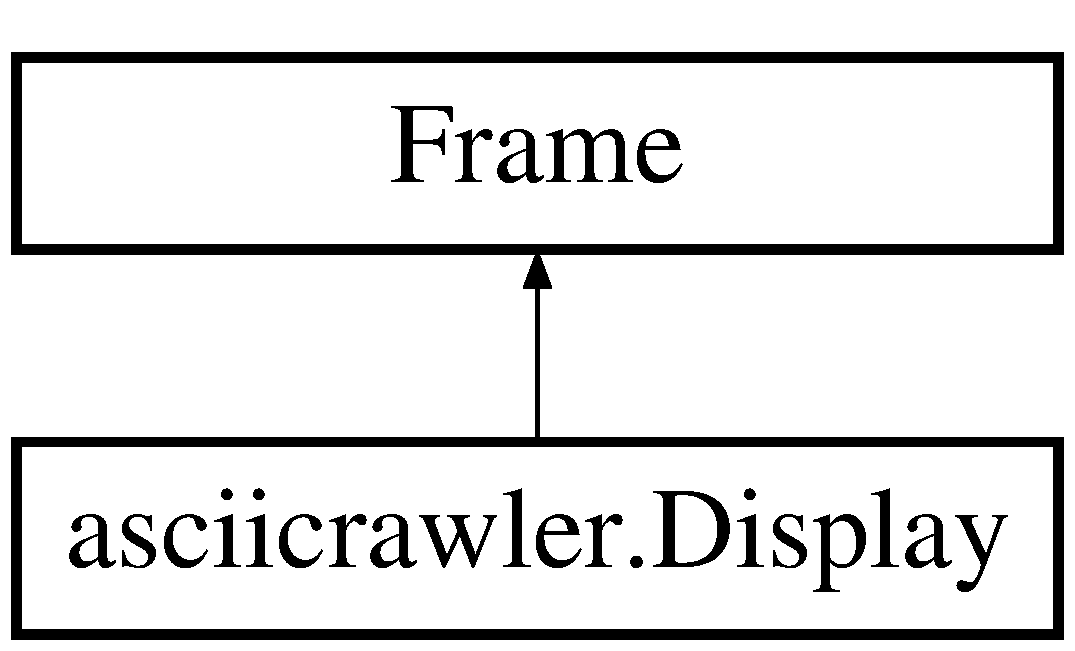
\includegraphics[height=2.000000cm]{classasciicrawler_1_1Display}
\end{center}
\end{figure}
\subsection*{Public Member Functions}
\begin{DoxyCompactItemize}
\item 
\hyperlink{classasciicrawler_1_1Display_a7141b4471b8b75b5c7da12769f4bf46c}{Display} (Window\+Adapter a, Key\+Listener b)
\item 
void \hyperlink{classasciicrawler_1_1Display_afbfb9296a48fa04d148715918230d3b2}{update\+Title} ()
\item 
void \hyperlink{classasciicrawler_1_1Display_ac78b41f2afc6b0732ab4cd54d7142604}{render\+Board} ()
\end{DoxyCompactItemize}


\subsection{Detailed Description}
Class is the display of the game and handles the rendering. 

\begin{DoxyAuthor}{Author}
Leon Hansen, Felix Schmidt 
\end{DoxyAuthor}
\begin{DoxyVersion}{Version}
1.\+0 
\end{DoxyVersion}


\subsection{Constructor \& Destructor Documentation}
\mbox{\Hypertarget{classasciicrawler_1_1Display_a7141b4471b8b75b5c7da12769f4bf46c}\label{classasciicrawler_1_1Display_a7141b4471b8b75b5c7da12769f4bf46c}} 
\index{asciicrawler\+::\+Display@{asciicrawler\+::\+Display}!Display@{Display}}
\index{Display@{Display}!asciicrawler\+::\+Display@{asciicrawler\+::\+Display}}
\subsubsection{\texorpdfstring{Display()}{Display()}}
{\footnotesize\ttfamily asciicrawler.\+Display.\+Display (\begin{DoxyParamCaption}\item[{Window\+Adapter}]{a,  }\item[{Key\+Listener}]{b }\end{DoxyParamCaption})\hspace{0.3cm}{\ttfamily [inline]}}

Constructor of the \hyperlink{classasciicrawler_1_1Display}{Display} class set the frame title and size


\begin{DoxyParams}{Parameters}
{\em a} & adapter which get the window events and one to listen to key presses\\
\hline
{\em b} & listener to recognize if any key was pressed \\
\hline
\end{DoxyParams}


\subsection{Member Function Documentation}
\mbox{\Hypertarget{classasciicrawler_1_1Display_ac78b41f2afc6b0732ab4cd54d7142604}\label{classasciicrawler_1_1Display_ac78b41f2afc6b0732ab4cd54d7142604}} 
\index{asciicrawler\+::\+Display@{asciicrawler\+::\+Display}!render\+Board@{render\+Board}}
\index{render\+Board@{render\+Board}!asciicrawler\+::\+Display@{asciicrawler\+::\+Display}}
\subsubsection{\texorpdfstring{render\+Board()}{renderBoard()}}
{\footnotesize\ttfamily void asciicrawler.\+Display.\+render\+Board (\begin{DoxyParamCaption}{ }\end{DoxyParamCaption})\hspace{0.3cm}{\ttfamily [inline]}}

renders the actual state of the board \mbox{\Hypertarget{classasciicrawler_1_1Display_afbfb9296a48fa04d148715918230d3b2}\label{classasciicrawler_1_1Display_afbfb9296a48fa04d148715918230d3b2}} 
\index{asciicrawler\+::\+Display@{asciicrawler\+::\+Display}!update\+Title@{update\+Title}}
\index{update\+Title@{update\+Title}!asciicrawler\+::\+Display@{asciicrawler\+::\+Display}}
\subsubsection{\texorpdfstring{update\+Title()}{updateTitle()}}
{\footnotesize\ttfamily void asciicrawler.\+Display.\+update\+Title (\begin{DoxyParamCaption}{ }\end{DoxyParamCaption})\hspace{0.3cm}{\ttfamily [inline]}}

provides information about the level and score on the updatetitle 

The documentation for this class was generated from the following file\+:\begin{DoxyCompactItemize}
\item 
/home/felix/\+Documents/\+Uni/\+Master/1. Semester/\+Technische Dokumentation/\+Spiel/\+Ascii-\/\+Crawler/src/asciicrawler/Display.\+java\end{DoxyCompactItemize}

\hypertarget{classasciicrawler_1_1Enemy}{}\section{asciicrawler.\+Enemy Class Reference}
\label{classasciicrawler_1_1Enemy}\index{asciicrawler.\+Enemy@{asciicrawler.\+Enemy}}


Contains the \hyperlink{classasciicrawler_1_1Enemy}{Enemy} AI.  


Inheritance diagram for asciicrawler.\+Enemy\+:\begin{figure}[H]
\begin{center}
\leavevmode
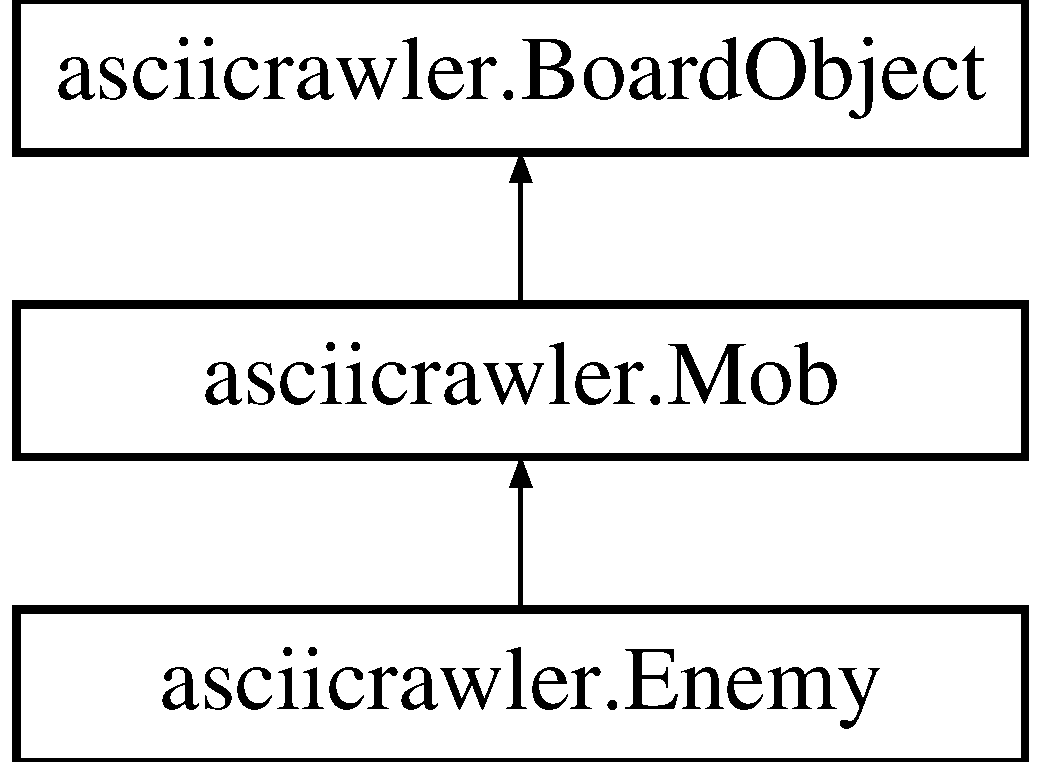
\includegraphics[height=3.000000cm]{classasciicrawler_1_1Enemy}
\end{center}
\end{figure}
\subsection*{Public Member Functions}
\begin{DoxyCompactItemize}
\item 
void \hyperlink{classasciicrawler_1_1Enemy_afe6ebef5eeb864014ca199659b075d49}{kill} ()
\item 
Color \hyperlink{classasciicrawler_1_1Enemy_a86551f4c55693124ea420002af778fdc}{get\+Color} ()
\item 
boolean \hyperlink{classasciicrawler_1_1Enemy_a278cb592e872c27a9faa8932f1c14819}{can\+See\+Player} (\hyperlink{enumasciicrawler_1_1Direction}{Direction} d)
\item 
void \hyperlink{classasciicrawler_1_1Enemy_afde325bd1c572dd3ff925b335be6ab0e}{move} ()
\end{DoxyCompactItemize}
\subsection*{Public Attributes}
\begin{DoxyCompactItemize}
\item 
int \hyperlink{classasciicrawler_1_1Enemy_a4521663e829959a7c25327925b8a8f40}{move\+Timer} = 50
\item 
\hyperlink{enumasciicrawler_1_1Direction}{Direction} \hyperlink{classasciicrawler_1_1Enemy_ab2fc6a3c9949c3d4317549f84a061ab9}{facing} = \hyperlink{enumasciicrawler_1_1Direction_a6ddc24b03c5e790038cb48cf48ed8bb0}{Direction.\+UP}
\item 
boolean \hyperlink{classasciicrawler_1_1Enemy_aed37076b976c543c6099e7a4199c8a18}{is\+Dead} = false
\end{DoxyCompactItemize}
\subsection*{Static Public Attributes}
\begin{DoxyCompactItemize}
\item 
static final int \hyperlink{classasciicrawler_1_1Enemy_a68c41f5b3ff03ce66a0a7748c6dcae31}{Charge\+Delay\+Min} = 6
\item 
static final int \hyperlink{classasciicrawler_1_1Enemy_a5d4281f4774665c377922b28bc53a142}{Charge\+Delay\+Random} = 3
\item 
static final int \hyperlink{classasciicrawler_1_1Enemy_a90ed20929053611dcb72a406b51d38c7}{Walk\+Delay\+Min} = 12
\item 
static final int \hyperlink{classasciicrawler_1_1Enemy_ab726ddd8887f94387edf105358a034a3}{Walk\+Delay\+Random} = 6
\item 
static final int \hyperlink{classasciicrawler_1_1Enemy_ac44d10fa43eb6b9507eb8876f52c0d28}{Death\+Time} = 500
\item 
static final int \hyperlink{classasciicrawler_1_1Enemy_a03cbf40a5f16e3023b00ece3bfe67554}{Waking\+Time} = 50
\end{DoxyCompactItemize}


\subsection{Detailed Description}
Contains the \hyperlink{classasciicrawler_1_1Enemy}{Enemy} AI. 

\begin{DoxyAuthor}{Author}
Leon Hansen, Felix Schmidt 
\end{DoxyAuthor}
\begin{DoxyVersion}{Version}
1.\+0 
\end{DoxyVersion}


\subsection{Member Function Documentation}
\mbox{\Hypertarget{classasciicrawler_1_1Enemy_a278cb592e872c27a9faa8932f1c14819}\label{classasciicrawler_1_1Enemy_a278cb592e872c27a9faa8932f1c14819}} 
\index{asciicrawler\+::\+Enemy@{asciicrawler\+::\+Enemy}!can\+See\+Player@{can\+See\+Player}}
\index{can\+See\+Player@{can\+See\+Player}!asciicrawler\+::\+Enemy@{asciicrawler\+::\+Enemy}}
\subsubsection{\texorpdfstring{can\+See\+Player()}{canSeePlayer()}}
{\footnotesize\ttfamily boolean asciicrawler.\+Enemy.\+can\+See\+Player (\begin{DoxyParamCaption}\item[{\hyperlink{enumasciicrawler_1_1Direction}{Direction}}]{d }\end{DoxyParamCaption})\hspace{0.3cm}{\ttfamily [inline]}}

Returns true when the enemy has no obstacles to the player in a given direction \mbox{\Hypertarget{classasciicrawler_1_1Enemy_a86551f4c55693124ea420002af778fdc}\label{classasciicrawler_1_1Enemy_a86551f4c55693124ea420002af778fdc}} 
\index{asciicrawler\+::\+Enemy@{asciicrawler\+::\+Enemy}!get\+Color@{get\+Color}}
\index{get\+Color@{get\+Color}!asciicrawler\+::\+Enemy@{asciicrawler\+::\+Enemy}}
\subsubsection{\texorpdfstring{get\+Color()}{getColor()}}
{\footnotesize\ttfamily Color asciicrawler.\+Enemy.\+get\+Color (\begin{DoxyParamCaption}{ }\end{DoxyParamCaption})\hspace{0.3cm}{\ttfamily [inline]}}

Returns the Color based on is\+Dead \mbox{\Hypertarget{classasciicrawler_1_1Enemy_afe6ebef5eeb864014ca199659b075d49}\label{classasciicrawler_1_1Enemy_afe6ebef5eeb864014ca199659b075d49}} 
\index{asciicrawler\+::\+Enemy@{asciicrawler\+::\+Enemy}!kill@{kill}}
\index{kill@{kill}!asciicrawler\+::\+Enemy@{asciicrawler\+::\+Enemy}}
\subsubsection{\texorpdfstring{kill()}{kill()}}
{\footnotesize\ttfamily void asciicrawler.\+Enemy.\+kill (\begin{DoxyParamCaption}{ }\end{DoxyParamCaption})\hspace{0.3cm}{\ttfamily [inline]}}

Set the resurrection timer and marks the \hyperlink{classasciicrawler_1_1Enemy}{Enemy} as dead \mbox{\Hypertarget{classasciicrawler_1_1Enemy_afde325bd1c572dd3ff925b335be6ab0e}\label{classasciicrawler_1_1Enemy_afde325bd1c572dd3ff925b335be6ab0e}} 
\index{asciicrawler\+::\+Enemy@{asciicrawler\+::\+Enemy}!move@{move}}
\index{move@{move}!asciicrawler\+::\+Enemy@{asciicrawler\+::\+Enemy}}
\subsubsection{\texorpdfstring{move()}{move()}}
{\footnotesize\ttfamily void asciicrawler.\+Enemy.\+move (\begin{DoxyParamCaption}{ }\end{DoxyParamCaption})\hspace{0.3cm}{\ttfamily [inline]}}

Called every game tick to move the enemy when necessary 

\subsection{Member Data Documentation}
\mbox{\Hypertarget{classasciicrawler_1_1Enemy_a68c41f5b3ff03ce66a0a7748c6dcae31}\label{classasciicrawler_1_1Enemy_a68c41f5b3ff03ce66a0a7748c6dcae31}} 
\index{asciicrawler\+::\+Enemy@{asciicrawler\+::\+Enemy}!Charge\+Delay\+Min@{Charge\+Delay\+Min}}
\index{Charge\+Delay\+Min@{Charge\+Delay\+Min}!asciicrawler\+::\+Enemy@{asciicrawler\+::\+Enemy}}
\subsubsection{\texorpdfstring{Charge\+Delay\+Min}{ChargeDelayMin}}
{\footnotesize\ttfamily final int asciicrawler.\+Enemy.\+Charge\+Delay\+Min = 6\hspace{0.3cm}{\ttfamily [static]}}

When \hyperlink{classasciicrawler_1_1Player}{Player} is in direct sight, this is the number of minimal ticks to the next move \mbox{\Hypertarget{classasciicrawler_1_1Enemy_a5d4281f4774665c377922b28bc53a142}\label{classasciicrawler_1_1Enemy_a5d4281f4774665c377922b28bc53a142}} 
\index{asciicrawler\+::\+Enemy@{asciicrawler\+::\+Enemy}!Charge\+Delay\+Random@{Charge\+Delay\+Random}}
\index{Charge\+Delay\+Random@{Charge\+Delay\+Random}!asciicrawler\+::\+Enemy@{asciicrawler\+::\+Enemy}}
\subsubsection{\texorpdfstring{Charge\+Delay\+Random}{ChargeDelayRandom}}
{\footnotesize\ttfamily final int asciicrawler.\+Enemy.\+Charge\+Delay\+Random = 3\hspace{0.3cm}{\ttfamily [static]}}

Difference in ticks of charging moves. Maximum delay is Min + Random -\/ 1 \mbox{\Hypertarget{classasciicrawler_1_1Enemy_ac44d10fa43eb6b9507eb8876f52c0d28}\label{classasciicrawler_1_1Enemy_ac44d10fa43eb6b9507eb8876f52c0d28}} 
\index{asciicrawler\+::\+Enemy@{asciicrawler\+::\+Enemy}!Death\+Time@{Death\+Time}}
\index{Death\+Time@{Death\+Time}!asciicrawler\+::\+Enemy@{asciicrawler\+::\+Enemy}}
\subsubsection{\texorpdfstring{Death\+Time}{DeathTime}}
{\footnotesize\ttfamily final int asciicrawler.\+Enemy.\+Death\+Time = 500\hspace{0.3cm}{\ttfamily [static]}}

Number of ticks it take an enemy to resurrect \mbox{\Hypertarget{classasciicrawler_1_1Enemy_ab2fc6a3c9949c3d4317549f84a061ab9}\label{classasciicrawler_1_1Enemy_ab2fc6a3c9949c3d4317549f84a061ab9}} 
\index{asciicrawler\+::\+Enemy@{asciicrawler\+::\+Enemy}!facing@{facing}}
\index{facing@{facing}!asciicrawler\+::\+Enemy@{asciicrawler\+::\+Enemy}}
\subsubsection{\texorpdfstring{facing}{facing}}
{\footnotesize\ttfamily \hyperlink{enumasciicrawler_1_1Direction}{Direction} asciicrawler.\+Enemy.\+facing = \hyperlink{enumasciicrawler_1_1Direction_a6ddc24b03c5e790038cb48cf48ed8bb0}{Direction.\+UP}}

Directions the enemy is looking at. It can only walk back when there is no alternative \mbox{\Hypertarget{classasciicrawler_1_1Enemy_aed37076b976c543c6099e7a4199c8a18}\label{classasciicrawler_1_1Enemy_aed37076b976c543c6099e7a4199c8a18}} 
\index{asciicrawler\+::\+Enemy@{asciicrawler\+::\+Enemy}!is\+Dead@{is\+Dead}}
\index{is\+Dead@{is\+Dead}!asciicrawler\+::\+Enemy@{asciicrawler\+::\+Enemy}}
\subsubsection{\texorpdfstring{is\+Dead}{isDead}}
{\footnotesize\ttfamily boolean asciicrawler.\+Enemy.\+is\+Dead = false}

Whether the \hyperlink{classasciicrawler_1_1Enemy}{Enemy} is alive and can move \mbox{\Hypertarget{classasciicrawler_1_1Enemy_a4521663e829959a7c25327925b8a8f40}\label{classasciicrawler_1_1Enemy_a4521663e829959a7c25327925b8a8f40}} 
\index{asciicrawler\+::\+Enemy@{asciicrawler\+::\+Enemy}!move\+Timer@{move\+Timer}}
\index{move\+Timer@{move\+Timer}!asciicrawler\+::\+Enemy@{asciicrawler\+::\+Enemy}}
\subsubsection{\texorpdfstring{move\+Timer}{moveTimer}}
{\footnotesize\ttfamily int asciicrawler.\+Enemy.\+move\+Timer = 50}

Number of ticks until the next move \mbox{\Hypertarget{classasciicrawler_1_1Enemy_a03cbf40a5f16e3023b00ece3bfe67554}\label{classasciicrawler_1_1Enemy_a03cbf40a5f16e3023b00ece3bfe67554}} 
\index{asciicrawler\+::\+Enemy@{asciicrawler\+::\+Enemy}!Waking\+Time@{Waking\+Time}}
\index{Waking\+Time@{Waking\+Time}!asciicrawler\+::\+Enemy@{asciicrawler\+::\+Enemy}}
\subsubsection{\texorpdfstring{Waking\+Time}{WakingTime}}
{\footnotesize\ttfamily final int asciicrawler.\+Enemy.\+Waking\+Time = 50\hspace{0.3cm}{\ttfamily [static]}}

Number of ticks the enemy does not move after resurrection \mbox{\Hypertarget{classasciicrawler_1_1Enemy_a90ed20929053611dcb72a406b51d38c7}\label{classasciicrawler_1_1Enemy_a90ed20929053611dcb72a406b51d38c7}} 
\index{asciicrawler\+::\+Enemy@{asciicrawler\+::\+Enemy}!Walk\+Delay\+Min@{Walk\+Delay\+Min}}
\index{Walk\+Delay\+Min@{Walk\+Delay\+Min}!asciicrawler\+::\+Enemy@{asciicrawler\+::\+Enemy}}
\subsubsection{\texorpdfstring{Walk\+Delay\+Min}{WalkDelayMin}}
{\footnotesize\ttfamily final int asciicrawler.\+Enemy.\+Walk\+Delay\+Min = 12\hspace{0.3cm}{\ttfamily [static]}}

When wandering around, this is the number of minimal ticks to the next move \mbox{\Hypertarget{classasciicrawler_1_1Enemy_ab726ddd8887f94387edf105358a034a3}\label{classasciicrawler_1_1Enemy_ab726ddd8887f94387edf105358a034a3}} 
\index{asciicrawler\+::\+Enemy@{asciicrawler\+::\+Enemy}!Walk\+Delay\+Random@{Walk\+Delay\+Random}}
\index{Walk\+Delay\+Random@{Walk\+Delay\+Random}!asciicrawler\+::\+Enemy@{asciicrawler\+::\+Enemy}}
\subsubsection{\texorpdfstring{Walk\+Delay\+Random}{WalkDelayRandom}}
{\footnotesize\ttfamily final int asciicrawler.\+Enemy.\+Walk\+Delay\+Random = 6\hspace{0.3cm}{\ttfamily [static]}}

Difference in ticks of walking moves. Maximum delay is Min + Random -\/ 1 

The documentation for this class was generated from the following file\+:\begin{DoxyCompactItemize}
\item 
/home/felix/\+Documents/\+Uni/\+Master/1. Semester/\+Technische Dokumentation/\+Spiel/\+Ascii-\/\+Crawler/src/asciicrawler/Enemy.\+java\end{DoxyCompactItemize}

\hypertarget{classasciicrawler_1_1Exit}{}\section{asciicrawler.\+Exit Class Reference}
\label{classasciicrawler_1_1Exit}\index{asciicrawler.\+Exit@{asciicrawler.\+Exit}}


\hyperlink{classasciicrawler_1_1Exit}{Exit} is a board object. It is the field in the game where the player starts and the ends the level.  


Inheritance diagram for asciicrawler.\+Exit\+:\begin{figure}[H]
\begin{center}
\leavevmode
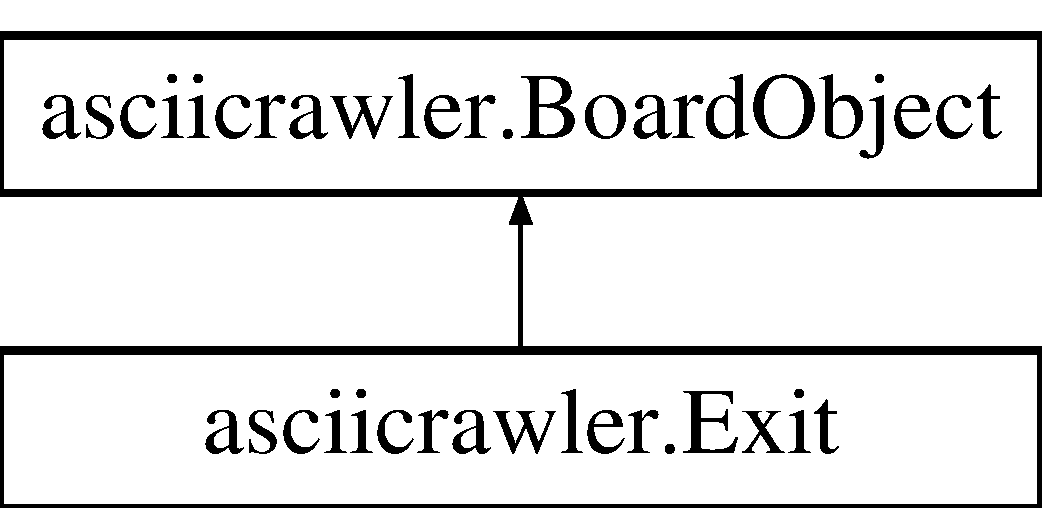
\includegraphics[height=2.000000cm]{classasciicrawler_1_1Exit}
\end{center}
\end{figure}
\subsection*{Public Member Functions}
\begin{DoxyCompactItemize}
\item 
boolean \hyperlink{classasciicrawler_1_1Exit_a38b93acb30670f4f4ba1c3059e0bbfa0}{can\+Enter} ()
\item 
Color \hyperlink{classasciicrawler_1_1Exit_a846df814b72bfab477c524427570d0cd}{get\+Color} ()
\item 
void \hyperlink{classasciicrawler_1_1Exit_adaf13dd0b5f3bb6cf25230da9dc166bc}{On\+Enter} ()
\end{DoxyCompactItemize}


\subsection{Detailed Description}
\hyperlink{classasciicrawler_1_1Exit}{Exit} is a board object. It is the field in the game where the player starts and the ends the level. 

\begin{DoxyAuthor}{Author}
Leon Hansen, Felix Schmidt 
\end{DoxyAuthor}
\begin{DoxyVersion}{Version}
1.\+0 
\end{DoxyVersion}


\subsection{Member Function Documentation}
\mbox{\Hypertarget{classasciicrawler_1_1Exit_a38b93acb30670f4f4ba1c3059e0bbfa0}\label{classasciicrawler_1_1Exit_a38b93acb30670f4f4ba1c3059e0bbfa0}} 
\index{asciicrawler\+::\+Exit@{asciicrawler\+::\+Exit}!can\+Enter@{can\+Enter}}
\index{can\+Enter@{can\+Enter}!asciicrawler\+::\+Exit@{asciicrawler\+::\+Exit}}
\subsubsection{\texorpdfstring{can\+Enter()}{canEnter()}}
{\footnotesize\ttfamily boolean asciicrawler.\+Exit.\+can\+Enter (\begin{DoxyParamCaption}{ }\end{DoxyParamCaption})\hspace{0.3cm}{\ttfamily [inline]}}

Checks if the \hyperlink{classasciicrawler_1_1Mob}{Mob} can access this type of field \mbox{\Hypertarget{classasciicrawler_1_1Exit_a846df814b72bfab477c524427570d0cd}\label{classasciicrawler_1_1Exit_a846df814b72bfab477c524427570d0cd}} 
\index{asciicrawler\+::\+Exit@{asciicrawler\+::\+Exit}!get\+Color@{get\+Color}}
\index{get\+Color@{get\+Color}!asciicrawler\+::\+Exit@{asciicrawler\+::\+Exit}}
\subsubsection{\texorpdfstring{get\+Color()}{getColor()}}
{\footnotesize\ttfamily Color asciicrawler.\+Exit.\+get\+Color (\begin{DoxyParamCaption}{ }\end{DoxyParamCaption})\hspace{0.3cm}{\ttfamily [inline]}}

Returns the Color of the field \mbox{\Hypertarget{classasciicrawler_1_1Exit_adaf13dd0b5f3bb6cf25230da9dc166bc}\label{classasciicrawler_1_1Exit_adaf13dd0b5f3bb6cf25230da9dc166bc}} 
\index{asciicrawler\+::\+Exit@{asciicrawler\+::\+Exit}!On\+Enter@{On\+Enter}}
\index{On\+Enter@{On\+Enter}!asciicrawler\+::\+Exit@{asciicrawler\+::\+Exit}}
\subsubsection{\texorpdfstring{On\+Enter()}{OnEnter()}}
{\footnotesize\ttfamily void asciicrawler.\+Exit.\+On\+Enter (\begin{DoxyParamCaption}{ }\end{DoxyParamCaption})\hspace{0.3cm}{\ttfamily [inline]}}

Defines which events (on condition) happens when the field is entered by a mob. 

The documentation for this class was generated from the following file\+:\begin{DoxyCompactItemize}
\item 
/home/felix/\+Documents/\+Uni/\+Master/1. Semester/\+Technische Dokumentation/\+Spiel/\+Ascii-\/\+Crawler/src/asciicrawler/Exit.\+java\end{DoxyCompactItemize}

\hypertarget{classasciicrawler_1_1Game}{}\section{asciicrawler.\+Game Class Reference}
\label{classasciicrawler_1_1Game}\index{asciicrawler.\+Game@{asciicrawler.\+Game}}
\subsection*{Static Public Member Functions}
\begin{DoxyCompactItemize}
\item 
\mbox{\Hypertarget{classasciicrawler_1_1Game_a710127c5e068bab243b8ae11b94eaf7e}\label{classasciicrawler_1_1Game_a710127c5e068bab243b8ae11b94eaf7e}} 
static void {\bfseries add\+Score} (int n)
\item 
\mbox{\Hypertarget{classasciicrawler_1_1Game_a3b40e9fa0de37e53daaaaf66d073f027}\label{classasciicrawler_1_1Game_a3b40e9fa0de37e53daaaaf66d073f027}} 
static void {\bfseries won} ()
\item 
\mbox{\Hypertarget{classasciicrawler_1_1Game_a8158267fd8ae418c716d9b4a12ab5881}\label{classasciicrawler_1_1Game_a8158267fd8ae418c716d9b4a12ab5881}} 
static void {\bfseries lost} ()
\end{DoxyCompactItemize}
\subsection*{Static Public Attributes}
\begin{DoxyCompactItemize}
\item 
\mbox{\Hypertarget{classasciicrawler_1_1Game_a88a2d61444df3841c2d6fbb6f7df8afd}\label{classasciicrawler_1_1Game_a88a2d61444df3841c2d6fbb6f7df8afd}} 
static \hyperlink{classasciicrawler_1_1Board}{Board} {\bfseries board}
\item 
\mbox{\Hypertarget{classasciicrawler_1_1Game_af4264767479e3f2e395e23e505bc7f24}\label{classasciicrawler_1_1Game_af4264767479e3f2e395e23e505bc7f24}} 
static \hyperlink{classasciicrawler_1_1KeyManager}{Key\+Manager} {\bfseries keys}
\item 
\mbox{\Hypertarget{classasciicrawler_1_1Game_a169f0d8231cf07ac0f1dcc12035159e9}\label{classasciicrawler_1_1Game_a169f0d8231cf07ac0f1dcc12035159e9}} 
static \hyperlink{classasciicrawler_1_1Display}{Display} {\bfseries display}
\item 
\mbox{\Hypertarget{classasciicrawler_1_1Game_aa82e45424ef5c303711e2f154de64e90}\label{classasciicrawler_1_1Game_aa82e45424ef5c303711e2f154de64e90}} 
static Random {\bfseries ai\+Random}
\item 
\mbox{\Hypertarget{classasciicrawler_1_1Game_a58220b697f299e457bbe6963f4010c0c}\label{classasciicrawler_1_1Game_a58220b697f299e457bbe6963f4010c0c}} 
static int {\bfseries score} = 0
\item 
\mbox{\Hypertarget{classasciicrawler_1_1Game_a490824e2d8ea8fb6ba08159367f73a68}\label{classasciicrawler_1_1Game_a490824e2d8ea8fb6ba08159367f73a68}} 
static int {\bfseries level} = 1
\item 
\mbox{\Hypertarget{classasciicrawler_1_1Game_a3207bf872db55d678cbb3889694d381d}\label{classasciicrawler_1_1Game_a3207bf872db55d678cbb3889694d381d}} 
static final int {\bfseries Attack\+Score} = -\/40
\item 
\mbox{\Hypertarget{classasciicrawler_1_1Game_a79655e520f3645c8a589689b2b7052dd}\label{classasciicrawler_1_1Game_a79655e520f3645c8a589689b2b7052dd}} 
static final int {\bfseries Move\+Score} = -\/1
\item 
\mbox{\Hypertarget{classasciicrawler_1_1Game_a39baf9450132d5991ff1f32e01134b17}\label{classasciicrawler_1_1Game_a39baf9450132d5991ff1f32e01134b17}} 
static final int {\bfseries Level\+Win} = 700
\item 
\mbox{\Hypertarget{classasciicrawler_1_1Game_aa5cdd6aaa0bd4f61a134135b0647ce03}\label{classasciicrawler_1_1Game_aa5cdd6aaa0bd4f61a134135b0647ce03}} 
static final int {\bfseries Kill\+Score} = 60
\item 
\mbox{\Hypertarget{classasciicrawler_1_1Game_ace48576550dbbab59420923b516da04f}\label{classasciicrawler_1_1Game_ace48576550dbbab59420923b516da04f}} 
static final int {\bfseries Gold\+Score} = 300
\item 
\mbox{\Hypertarget{classasciicrawler_1_1Game_a7e2f14df631aefe04e9f7acd4e39abb2}\label{classasciicrawler_1_1Game_a7e2f14df631aefe04e9f7acd4e39abb2}} 
static Linked\+List$<$ Integer $>$ {\bfseries score\+Board}
\end{DoxyCompactItemize}


\subsection{Detailed Description}
\hyperlink{classMain}{Main} class of the game, Creates all components

\begin{DoxyAuthor}{Author}
Leon Hansen, Felix Schmidt 
\end{DoxyAuthor}
\begin{DoxyVersion}{Version}
1.\+0 
\end{DoxyVersion}


The documentation for this class was generated from the following file\+:\begin{DoxyCompactItemize}
\item 
/home/felix/\+Documents/\+Uni/\+Master/1. Semester/\+Technische Dokumentation/\+Spiel/\+Ascii-\/\+Crawler/src/asciicrawler/Game.\+java\end{DoxyCompactItemize}

\hypertarget{classasciicrawler_1_1GameTicker}{}\section{asciicrawler.\+Game\+Ticker Class Reference}
\label{classasciicrawler_1_1GameTicker}\index{asciicrawler.\+Game\+Ticker@{asciicrawler.\+Game\+Ticker}}


this will handle all game ticks and the movement of player/enemy  


Inheritance diagram for asciicrawler.\+Game\+Ticker\+:\begin{figure}[H]
\begin{center}
\leavevmode
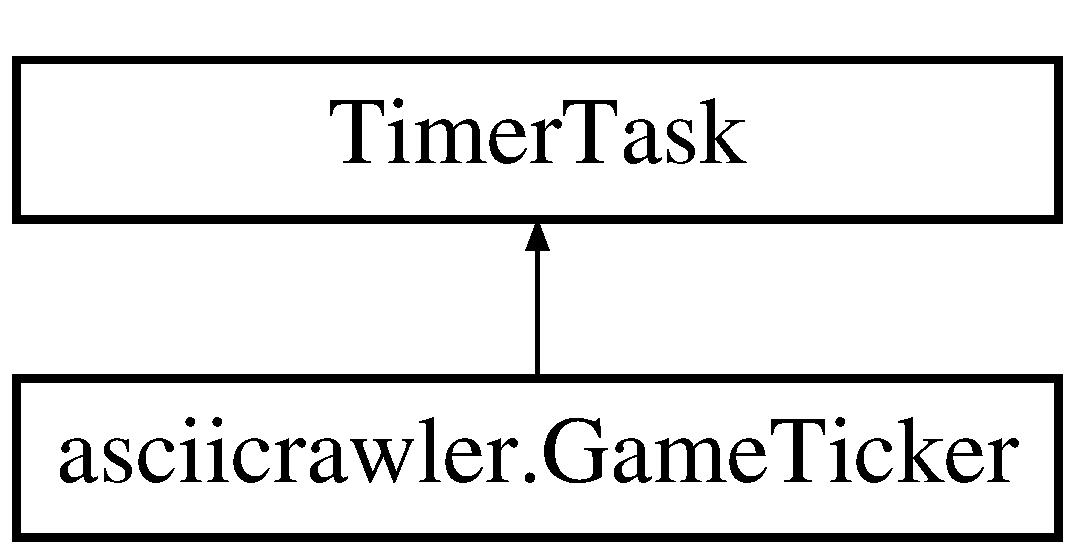
\includegraphics[height=2.000000cm]{classasciicrawler_1_1GameTicker}
\end{center}
\end{figure}
\subsection*{Public Member Functions}
\begin{DoxyCompactItemize}
\item 
void \hyperlink{classasciicrawler_1_1GameTicker_ace7f637461d8fde2033d01a2fc769275}{run} ()
\end{DoxyCompactItemize}


\subsection{Detailed Description}
this will handle all game ticks and the movement of player/enemy 

\begin{DoxyAuthor}{Author}
Leon Hansen, Felix Schmidt 
\end{DoxyAuthor}
\begin{DoxyVersion}{Version}
1.\+0 
\end{DoxyVersion}


\subsection{Member Function Documentation}
\mbox{\Hypertarget{classasciicrawler_1_1GameTicker_ace7f637461d8fde2033d01a2fc769275}\label{classasciicrawler_1_1GameTicker_ace7f637461d8fde2033d01a2fc769275}} 
\index{asciicrawler\+::\+Game\+Ticker@{asciicrawler\+::\+Game\+Ticker}!run@{run}}
\index{run@{run}!asciicrawler\+::\+Game\+Ticker@{asciicrawler\+::\+Game\+Ticker}}
\subsubsection{\texorpdfstring{run()}{run()}}
{\footnotesize\ttfamily void asciicrawler.\+Game\+Ticker.\+run (\begin{DoxyParamCaption}{ }\end{DoxyParamCaption})\hspace{0.3cm}{\ttfamily [inline]}}

handles the movement of all mobs in a defined frequence 

The documentation for this class was generated from the following file\+:\begin{DoxyCompactItemize}
\item 
/home/felix/\+Documents/\+Uni/\+Master/1. Semester/\+Technische Dokumentation/\+Spiel/\+Ascii-\/\+Crawler/src/asciicrawler/Game\+Ticker.\+java\end{DoxyCompactItemize}

\hypertarget{classasciicrawler_1_1Gold}{}\section{asciicrawler.\+Gold Class Reference}
\label{classasciicrawler_1_1Gold}\index{asciicrawler.\+Gold@{asciicrawler.\+Gold}}


\hyperlink{classasciicrawler_1_1Gold}{Gold} is a board object. The \hyperlink{classasciicrawler_1_1Player}{Player} have to reach this field one time and then he can go back to the Exit-\/field.  


Inheritance diagram for asciicrawler.\+Gold\+:\begin{figure}[H]
\begin{center}
\leavevmode
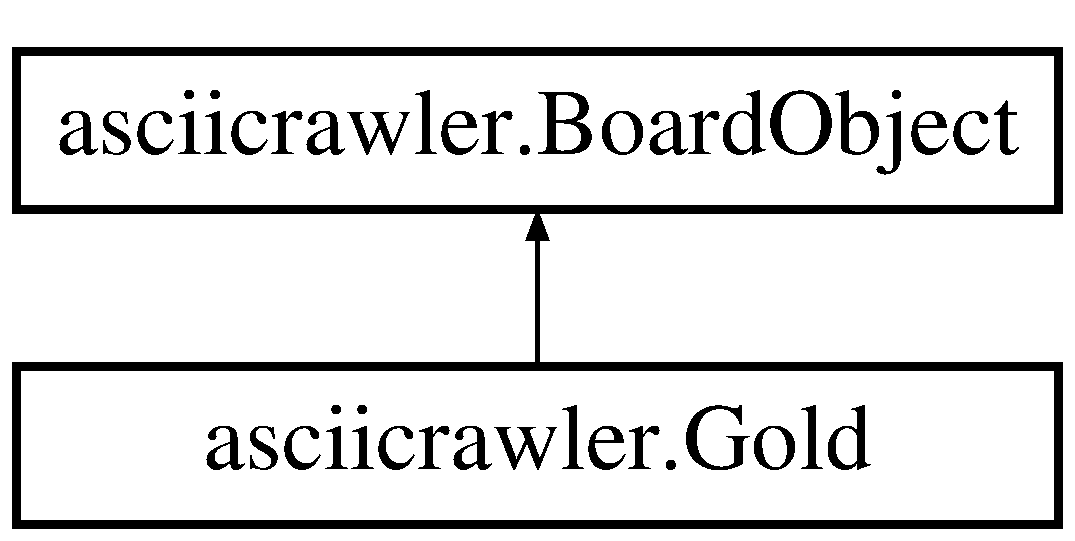
\includegraphics[height=2.000000cm]{classasciicrawler_1_1Gold}
\end{center}
\end{figure}
\subsection*{Public Member Functions}
\begin{DoxyCompactItemize}
\item 
boolean \hyperlink{classasciicrawler_1_1Gold_a383c92b41ae941567353150c3fc5c9b3}{can\+Enter} ()
\item 
Color \hyperlink{classasciicrawler_1_1Gold_a52713aa4b67ea23f2b729bb17034eb9e}{get\+Color} ()
\item 
void \hyperlink{classasciicrawler_1_1Gold_a663ee19ca7e6f0b0b518bd977df8b97b}{On\+Enter} ()
\end{DoxyCompactItemize}


\subsection{Detailed Description}
\hyperlink{classasciicrawler_1_1Gold}{Gold} is a board object. The \hyperlink{classasciicrawler_1_1Player}{Player} have to reach this field one time and then he can go back to the Exit-\/field. 

\begin{DoxyAuthor}{Author}
Leon Hansen, Felix Schmidt 
\end{DoxyAuthor}
\begin{DoxyVersion}{Version}
1.\+0 
\end{DoxyVersion}


\subsection{Member Function Documentation}
\mbox{\Hypertarget{classasciicrawler_1_1Gold_a383c92b41ae941567353150c3fc5c9b3}\label{classasciicrawler_1_1Gold_a383c92b41ae941567353150c3fc5c9b3}} 
\index{asciicrawler\+::\+Gold@{asciicrawler\+::\+Gold}!can\+Enter@{can\+Enter}}
\index{can\+Enter@{can\+Enter}!asciicrawler\+::\+Gold@{asciicrawler\+::\+Gold}}
\subsubsection{\texorpdfstring{can\+Enter()}{canEnter()}}
{\footnotesize\ttfamily boolean asciicrawler.\+Gold.\+can\+Enter (\begin{DoxyParamCaption}{ }\end{DoxyParamCaption})\hspace{0.3cm}{\ttfamily [inline]}}

Checks if the \hyperlink{classasciicrawler_1_1Mob}{Mob} can access this type of field \mbox{\Hypertarget{classasciicrawler_1_1Gold_a52713aa4b67ea23f2b729bb17034eb9e}\label{classasciicrawler_1_1Gold_a52713aa4b67ea23f2b729bb17034eb9e}} 
\index{asciicrawler\+::\+Gold@{asciicrawler\+::\+Gold}!get\+Color@{get\+Color}}
\index{get\+Color@{get\+Color}!asciicrawler\+::\+Gold@{asciicrawler\+::\+Gold}}
\subsubsection{\texorpdfstring{get\+Color()}{getColor()}}
{\footnotesize\ttfamily Color asciicrawler.\+Gold.\+get\+Color (\begin{DoxyParamCaption}{ }\end{DoxyParamCaption})\hspace{0.3cm}{\ttfamily [inline]}}

Returns the Color of the field \mbox{\Hypertarget{classasciicrawler_1_1Gold_a663ee19ca7e6f0b0b518bd977df8b97b}\label{classasciicrawler_1_1Gold_a663ee19ca7e6f0b0b518bd977df8b97b}} 
\index{asciicrawler\+::\+Gold@{asciicrawler\+::\+Gold}!On\+Enter@{On\+Enter}}
\index{On\+Enter@{On\+Enter}!asciicrawler\+::\+Gold@{asciicrawler\+::\+Gold}}
\subsubsection{\texorpdfstring{On\+Enter()}{OnEnter()}}
{\footnotesize\ttfamily void asciicrawler.\+Gold.\+On\+Enter (\begin{DoxyParamCaption}{ }\end{DoxyParamCaption})\hspace{0.3cm}{\ttfamily [inline]}}

Defines which events (on condition) happens when the field is entered by a mob. 

The documentation for this class was generated from the following file\+:\begin{DoxyCompactItemize}
\item 
/home/felix/\+Documents/\+Uni/\+Master/1. Semester/\+Technische Dokumentation/\+Spiel/\+Ascii-\/\+Crawler/src/asciicrawler/Gold.\+java\end{DoxyCompactItemize}

\hypertarget{classasciicrawler_1_1KeyManager}{}\section{asciicrawler.\+Key\+Manager Class Reference}
\label{classasciicrawler_1_1KeyManager}\index{asciicrawler.\+Key\+Manager@{asciicrawler.\+Key\+Manager}}


Mangaer to assign actions to specific key events.  


\subsection*{Public Member Functions}
\begin{DoxyCompactItemize}
\item 
synchronized void \hyperlink{classasciicrawler_1_1KeyManager_a891959638b2c091d79b2401587198511}{set\+Key} (int key)
\item 
synchronized \hyperlink{enumasciicrawler_1_1Direction}{Direction} \hyperlink{classasciicrawler_1_1KeyManager_a773bb4adf1be2cbb0584529f1945bb26}{get\+Move\+Request} ()
\item 
synchronized \hyperlink{enumasciicrawler_1_1Direction}{Direction} \hyperlink{classasciicrawler_1_1KeyManager_aea5d8fd872321b459ca769298476f377}{consume\+Move\+Request} ()
\item 
synchronized boolean \hyperlink{classasciicrawler_1_1KeyManager_a31c68dfad3df7fdc53e613ce90312be8}{consume\+Attack} ()
\end{DoxyCompactItemize}


\subsection{Detailed Description}
Mangaer to assign actions to specific key events. 

\begin{DoxyAuthor}{Author}
Leon Hansen, Felix Schmidt 
\end{DoxyAuthor}
\begin{DoxyVersion}{Version}
1.\+0 
\end{DoxyVersion}


\subsection{Member Function Documentation}
\mbox{\Hypertarget{classasciicrawler_1_1KeyManager_a31c68dfad3df7fdc53e613ce90312be8}\label{classasciicrawler_1_1KeyManager_a31c68dfad3df7fdc53e613ce90312be8}} 
\index{asciicrawler\+::\+Key\+Manager@{asciicrawler\+::\+Key\+Manager}!consume\+Attack@{consume\+Attack}}
\index{consume\+Attack@{consume\+Attack}!asciicrawler\+::\+Key\+Manager@{asciicrawler\+::\+Key\+Manager}}
\subsubsection{\texorpdfstring{consume\+Attack()}{consumeAttack()}}
{\footnotesize\ttfamily synchronized boolean asciicrawler.\+Key\+Manager.\+consume\+Attack (\begin{DoxyParamCaption}{ }\end{DoxyParamCaption})\hspace{0.3cm}{\ttfamily [inline]}}

returns if the player was attacking \mbox{\Hypertarget{classasciicrawler_1_1KeyManager_aea5d8fd872321b459ca769298476f377}\label{classasciicrawler_1_1KeyManager_aea5d8fd872321b459ca769298476f377}} 
\index{asciicrawler\+::\+Key\+Manager@{asciicrawler\+::\+Key\+Manager}!consume\+Move\+Request@{consume\+Move\+Request}}
\index{consume\+Move\+Request@{consume\+Move\+Request}!asciicrawler\+::\+Key\+Manager@{asciicrawler\+::\+Key\+Manager}}
\subsubsection{\texorpdfstring{consume\+Move\+Request()}{consumeMoveRequest()}}
{\footnotesize\ttfamily synchronized \hyperlink{enumasciicrawler_1_1Direction}{Direction} asciicrawler.\+Key\+Manager.\+consume\+Move\+Request (\begin{DoxyParamCaption}{ }\end{DoxyParamCaption})\hspace{0.3cm}{\ttfamily [inline]}}

returns the last movement \mbox{\Hypertarget{classasciicrawler_1_1KeyManager_a773bb4adf1be2cbb0584529f1945bb26}\label{classasciicrawler_1_1KeyManager_a773bb4adf1be2cbb0584529f1945bb26}} 
\index{asciicrawler\+::\+Key\+Manager@{asciicrawler\+::\+Key\+Manager}!get\+Move\+Request@{get\+Move\+Request}}
\index{get\+Move\+Request@{get\+Move\+Request}!asciicrawler\+::\+Key\+Manager@{asciicrawler\+::\+Key\+Manager}}
\subsubsection{\texorpdfstring{get\+Move\+Request()}{getMoveRequest()}}
{\footnotesize\ttfamily synchronized \hyperlink{enumasciicrawler_1_1Direction}{Direction} asciicrawler.\+Key\+Manager.\+get\+Move\+Request (\begin{DoxyParamCaption}{ }\end{DoxyParamCaption})\hspace{0.3cm}{\ttfamily [inline]}}

requests an update for moving \mbox{\Hypertarget{classasciicrawler_1_1KeyManager_a891959638b2c091d79b2401587198511}\label{classasciicrawler_1_1KeyManager_a891959638b2c091d79b2401587198511}} 
\index{asciicrawler\+::\+Key\+Manager@{asciicrawler\+::\+Key\+Manager}!set\+Key@{set\+Key}}
\index{set\+Key@{set\+Key}!asciicrawler\+::\+Key\+Manager@{asciicrawler\+::\+Key\+Manager}}
\subsubsection{\texorpdfstring{set\+Key()}{setKey()}}
{\footnotesize\ttfamily synchronized void asciicrawler.\+Key\+Manager.\+set\+Key (\begin{DoxyParamCaption}\item[{int}]{key }\end{DoxyParamCaption})\hspace{0.3cm}{\ttfamily [inline]}}

assign a action to a specific key 

The documentation for this class was generated from the following file\+:\begin{DoxyCompactItemize}
\item 
/home/felix/\+Documents/\+Uni/\+Master/1. Semester/\+Technische Dokumentation/\+Spiel/\+Ascii-\/\+Crawler/src/asciicrawler/Key\+Manager.\+java\end{DoxyCompactItemize}

\hypertarget{classMain}{}\section{Main Class Reference}
\label{classMain}\index{Main@{Main}}
\subsection*{Static Public Member Functions}
\begin{DoxyCompactItemize}
\item 
static void \hyperlink{classMain_a8a5d0f827edddff706cc0e6740d0579a}{main} (String\mbox{[}$\,$\mbox{]} args)
\end{DoxyCompactItemize}


\subsection{Detailed Description}
Creates the game

\begin{DoxyAuthor}{Author}
Leon Hansen, Felix Schmidt 
\end{DoxyAuthor}
\begin{DoxyVersion}{Version}
1.\+0 
\end{DoxyVersion}


\subsection{Member Function Documentation}
\mbox{\Hypertarget{classMain_a8a5d0f827edddff706cc0e6740d0579a}\label{classMain_a8a5d0f827edddff706cc0e6740d0579a}} 
\index{Main@{Main}!main@{main}}
\index{main@{main}!Main@{Main}}
\subsubsection{\texorpdfstring{main()}{main()}}
{\footnotesize\ttfamily static void Main.\+main (\begin{DoxyParamCaption}\item[{String \mbox{[}$\,$\mbox{]}}]{args }\end{DoxyParamCaption})\hspace{0.3cm}{\ttfamily [inline]}, {\ttfamily [static]}}

main method of the game ascii crawler 

The documentation for this class was generated from the following file\+:\begin{DoxyCompactItemize}
\item 
/home/felix/\+Documents/\+Uni/\+Master/1. Semester/\+Technische Dokumentation/\+Spiel/\+Ascii-\/\+Crawler/src/Main.\+java\end{DoxyCompactItemize}

\hypertarget{classasciicrawler_1_1Mob}{}\section{asciicrawler.\+Mob Class Reference}
\label{classasciicrawler_1_1Mob}\index{asciicrawler.\+Mob@{asciicrawler.\+Mob}}


Is the abstract class of several mob objects.  


Inheritance diagram for asciicrawler.\+Mob\+:\begin{figure}[H]
\begin{center}
\leavevmode
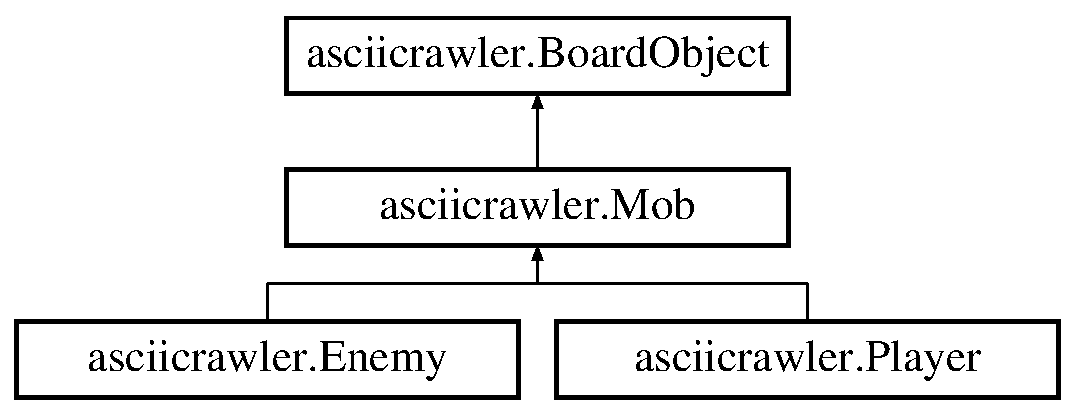
\includegraphics[height=3.000000cm]{classasciicrawler_1_1Mob}
\end{center}
\end{figure}
\subsection*{Public Member Functions}
\begin{DoxyCompactItemize}
\item 
int \hyperlink{classasciicrawler_1_1Mob_a10163bd48f4b365f0921a8b65f563017}{get\+X\+Position} ()
\item 
int \hyperlink{classasciicrawler_1_1Mob_a39572c2eb4a9dee3b92bd8094afffa9c}{get\+Y\+Position} ()
\item 
void \hyperlink{classasciicrawler_1_1Mob_a9029cbfef7c48ed085d387d8d6b0729d}{spawn\+At} (int x, int y)
\item 
boolean \hyperlink{classasciicrawler_1_1Mob_a494c5ae18f448b3dd98e7147d6e4c3db}{can\+Move\+To} (int x, int y)
\item 
boolean \hyperlink{classasciicrawler_1_1Mob_aee5629a34d8789bbec9918326fdd9612}{can\+Move\+In\+Direction} (\hyperlink{enumasciicrawler_1_1Direction}{Direction} d)
\item 
boolean \hyperlink{classasciicrawler_1_1Mob_a5f48e61e860b75d4de72e08321eaefed}{move\+To} (int x, int y)
\item 
boolean \hyperlink{classasciicrawler_1_1Mob_a2f215e78034f453c0769e04d5676384c}{move\+In\+Direction} (\hyperlink{enumasciicrawler_1_1Direction}{Direction} d)
\item 
boolean \hyperlink{classasciicrawler_1_1Mob_ad9f62c59a65cb1e8ab2f54d5a8e2fbe3}{can\+Enter} ()
\item 
abstract void \hyperlink{classasciicrawler_1_1Mob_a63b3e36b978aa3355d02e4a0b0906b0b}{move} ()
\end{DoxyCompactItemize}
\subsection*{Public Attributes}
\begin{DoxyCompactItemize}
\item 
boolean \hyperlink{classasciicrawler_1_1Mob_af8410e28e76e9507a9c96c7012ff3c91}{has\+Item} = false
\item 
\hyperlink{classasciicrawler_1_1BoardObject}{Board\+Object} \hyperlink{classasciicrawler_1_1Mob_a5682718b4d9809cfcc1010629f1ee0c7}{standing\+On}
\end{DoxyCompactItemize}


\subsection{Detailed Description}
Is the abstract class of several mob objects. 

\begin{DoxyAuthor}{Author}
Leon Hansen, Felix Schmidt 
\end{DoxyAuthor}
\begin{DoxyVersion}{Version}
1.\+0 
\end{DoxyVersion}


\subsection{Member Function Documentation}
\mbox{\Hypertarget{classasciicrawler_1_1Mob_ad9f62c59a65cb1e8ab2f54d5a8e2fbe3}\label{classasciicrawler_1_1Mob_ad9f62c59a65cb1e8ab2f54d5a8e2fbe3}} 
\index{asciicrawler\+::\+Mob@{asciicrawler\+::\+Mob}!can\+Enter@{can\+Enter}}
\index{can\+Enter@{can\+Enter}!asciicrawler\+::\+Mob@{asciicrawler\+::\+Mob}}
\subsubsection{\texorpdfstring{can\+Enter()}{canEnter()}}
{\footnotesize\ttfamily boolean asciicrawler.\+Mob.\+can\+Enter (\begin{DoxyParamCaption}{ }\end{DoxyParamCaption})\hspace{0.3cm}{\ttfamily [inline]}}

sets if an other mob can access the field \mbox{\Hypertarget{classasciicrawler_1_1Mob_aee5629a34d8789bbec9918326fdd9612}\label{classasciicrawler_1_1Mob_aee5629a34d8789bbec9918326fdd9612}} 
\index{asciicrawler\+::\+Mob@{asciicrawler\+::\+Mob}!can\+Move\+In\+Direction@{can\+Move\+In\+Direction}}
\index{can\+Move\+In\+Direction@{can\+Move\+In\+Direction}!asciicrawler\+::\+Mob@{asciicrawler\+::\+Mob}}
\subsubsection{\texorpdfstring{can\+Move\+In\+Direction()}{canMoveInDirection()}}
{\footnotesize\ttfamily boolean asciicrawler.\+Mob.\+can\+Move\+In\+Direction (\begin{DoxyParamCaption}\item[{\hyperlink{enumasciicrawler_1_1Direction}{Direction}}]{d }\end{DoxyParamCaption})\hspace{0.3cm}{\ttfamily [inline]}}

checks if a mob can move to a specific direction \mbox{\Hypertarget{classasciicrawler_1_1Mob_a494c5ae18f448b3dd98e7147d6e4c3db}\label{classasciicrawler_1_1Mob_a494c5ae18f448b3dd98e7147d6e4c3db}} 
\index{asciicrawler\+::\+Mob@{asciicrawler\+::\+Mob}!can\+Move\+To@{can\+Move\+To}}
\index{can\+Move\+To@{can\+Move\+To}!asciicrawler\+::\+Mob@{asciicrawler\+::\+Mob}}
\subsubsection{\texorpdfstring{can\+Move\+To()}{canMoveTo()}}
{\footnotesize\ttfamily boolean asciicrawler.\+Mob.\+can\+Move\+To (\begin{DoxyParamCaption}\item[{int}]{x,  }\item[{int}]{y }\end{DoxyParamCaption})\hspace{0.3cm}{\ttfamily [inline]}}

checks if a mob can move to a specific field \mbox{\Hypertarget{classasciicrawler_1_1Mob_a10163bd48f4b365f0921a8b65f563017}\label{classasciicrawler_1_1Mob_a10163bd48f4b365f0921a8b65f563017}} 
\index{asciicrawler\+::\+Mob@{asciicrawler\+::\+Mob}!get\+X\+Position@{get\+X\+Position}}
\index{get\+X\+Position@{get\+X\+Position}!asciicrawler\+::\+Mob@{asciicrawler\+::\+Mob}}
\subsubsection{\texorpdfstring{get\+X\+Position()}{getXPosition()}}
{\footnotesize\ttfamily int asciicrawler.\+Mob.\+get\+X\+Position (\begin{DoxyParamCaption}{ }\end{DoxyParamCaption})\hspace{0.3cm}{\ttfamily [inline]}}

returns the actual x Position of a mob \mbox{\Hypertarget{classasciicrawler_1_1Mob_a39572c2eb4a9dee3b92bd8094afffa9c}\label{classasciicrawler_1_1Mob_a39572c2eb4a9dee3b92bd8094afffa9c}} 
\index{asciicrawler\+::\+Mob@{asciicrawler\+::\+Mob}!get\+Y\+Position@{get\+Y\+Position}}
\index{get\+Y\+Position@{get\+Y\+Position}!asciicrawler\+::\+Mob@{asciicrawler\+::\+Mob}}
\subsubsection{\texorpdfstring{get\+Y\+Position()}{getYPosition()}}
{\footnotesize\ttfamily int asciicrawler.\+Mob.\+get\+Y\+Position (\begin{DoxyParamCaption}{ }\end{DoxyParamCaption})\hspace{0.3cm}{\ttfamily [inline]}}

returns the actual x Position of a mob \mbox{\Hypertarget{classasciicrawler_1_1Mob_a63b3e36b978aa3355d02e4a0b0906b0b}\label{classasciicrawler_1_1Mob_a63b3e36b978aa3355d02e4a0b0906b0b}} 
\index{asciicrawler\+::\+Mob@{asciicrawler\+::\+Mob}!move@{move}}
\index{move@{move}!asciicrawler\+::\+Mob@{asciicrawler\+::\+Mob}}
\subsubsection{\texorpdfstring{move()}{move()}}
{\footnotesize\ttfamily abstract void asciicrawler.\+Mob.\+move (\begin{DoxyParamCaption}{ }\end{DoxyParamCaption})\hspace{0.3cm}{\ttfamily [abstract]}}

abstract method to define the movement of a mob \mbox{\Hypertarget{classasciicrawler_1_1Mob_a2f215e78034f453c0769e04d5676384c}\label{classasciicrawler_1_1Mob_a2f215e78034f453c0769e04d5676384c}} 
\index{asciicrawler\+::\+Mob@{asciicrawler\+::\+Mob}!move\+In\+Direction@{move\+In\+Direction}}
\index{move\+In\+Direction@{move\+In\+Direction}!asciicrawler\+::\+Mob@{asciicrawler\+::\+Mob}}
\subsubsection{\texorpdfstring{move\+In\+Direction()}{moveInDirection()}}
{\footnotesize\ttfamily boolean asciicrawler.\+Mob.\+move\+In\+Direction (\begin{DoxyParamCaption}\item[{\hyperlink{enumasciicrawler_1_1Direction}{Direction}}]{d }\end{DoxyParamCaption})\hspace{0.3cm}{\ttfamily [inline]}}

sets the walking direction of a mob \mbox{\Hypertarget{classasciicrawler_1_1Mob_a5f48e61e860b75d4de72e08321eaefed}\label{classasciicrawler_1_1Mob_a5f48e61e860b75d4de72e08321eaefed}} 
\index{asciicrawler\+::\+Mob@{asciicrawler\+::\+Mob}!move\+To@{move\+To}}
\index{move\+To@{move\+To}!asciicrawler\+::\+Mob@{asciicrawler\+::\+Mob}}
\subsubsection{\texorpdfstring{move\+To()}{moveTo()}}
{\footnotesize\ttfamily boolean asciicrawler.\+Mob.\+move\+To (\begin{DoxyParamCaption}\item[{int}]{x,  }\item[{int}]{y }\end{DoxyParamCaption})\hspace{0.3cm}{\ttfamily [inline]}}

moves a mob to specific field \mbox{\Hypertarget{classasciicrawler_1_1Mob_a9029cbfef7c48ed085d387d8d6b0729d}\label{classasciicrawler_1_1Mob_a9029cbfef7c48ed085d387d8d6b0729d}} 
\index{asciicrawler\+::\+Mob@{asciicrawler\+::\+Mob}!spawn\+At@{spawn\+At}}
\index{spawn\+At@{spawn\+At}!asciicrawler\+::\+Mob@{asciicrawler\+::\+Mob}}
\subsubsection{\texorpdfstring{spawn\+At()}{spawnAt()}}
{\footnotesize\ttfamily void asciicrawler.\+Mob.\+spawn\+At (\begin{DoxyParamCaption}\item[{int}]{x,  }\item[{int}]{y }\end{DoxyParamCaption})\hspace{0.3cm}{\ttfamily [inline]}}

sets the spawn point of a mob 

\subsection{Member Data Documentation}
\mbox{\Hypertarget{classasciicrawler_1_1Mob_af8410e28e76e9507a9c96c7012ff3c91}\label{classasciicrawler_1_1Mob_af8410e28e76e9507a9c96c7012ff3c91}} 
\index{asciicrawler\+::\+Mob@{asciicrawler\+::\+Mob}!has\+Item@{has\+Item}}
\index{has\+Item@{has\+Item}!asciicrawler\+::\+Mob@{asciicrawler\+::\+Mob}}
\subsubsection{\texorpdfstring{has\+Item}{hasItem}}
{\footnotesize\ttfamily boolean asciicrawler.\+Mob.\+has\+Item = false}

state if mob has an item \mbox{\Hypertarget{classasciicrawler_1_1Mob_a5682718b4d9809cfcc1010629f1ee0c7}\label{classasciicrawler_1_1Mob_a5682718b4d9809cfcc1010629f1ee0c7}} 
\index{asciicrawler\+::\+Mob@{asciicrawler\+::\+Mob}!standing\+On@{standing\+On}}
\index{standing\+On@{standing\+On}!asciicrawler\+::\+Mob@{asciicrawler\+::\+Mob}}
\subsubsection{\texorpdfstring{standing\+On}{standingOn}}
{\footnotesize\ttfamily \hyperlink{classasciicrawler_1_1BoardObject}{Board\+Object} asciicrawler.\+Mob.\+standing\+On}

type of the board object the mob is standing on 

The documentation for this class was generated from the following file\+:\begin{DoxyCompactItemize}
\item 
/home/felix/\+Documents/\+Uni/\+Master/1. Semester/\+Technische Dokumentation/\+Spiel/\+Ascii-\/\+Crawler/src/asciicrawler/Mob.\+java\end{DoxyCompactItemize}

\hypertarget{classasciicrawler_1_1Player}{}\section{asciicrawler.\+Player Class Reference}
\label{classasciicrawler_1_1Player}\index{asciicrawler.\+Player@{asciicrawler.\+Player}}


\hyperlink{classasciicrawler_1_1Player}{Player} is class derived from mob. It specifices the abilities and and actions of a player.  


Inheritance diagram for asciicrawler.\+Player\+:\begin{figure}[H]
\begin{center}
\leavevmode
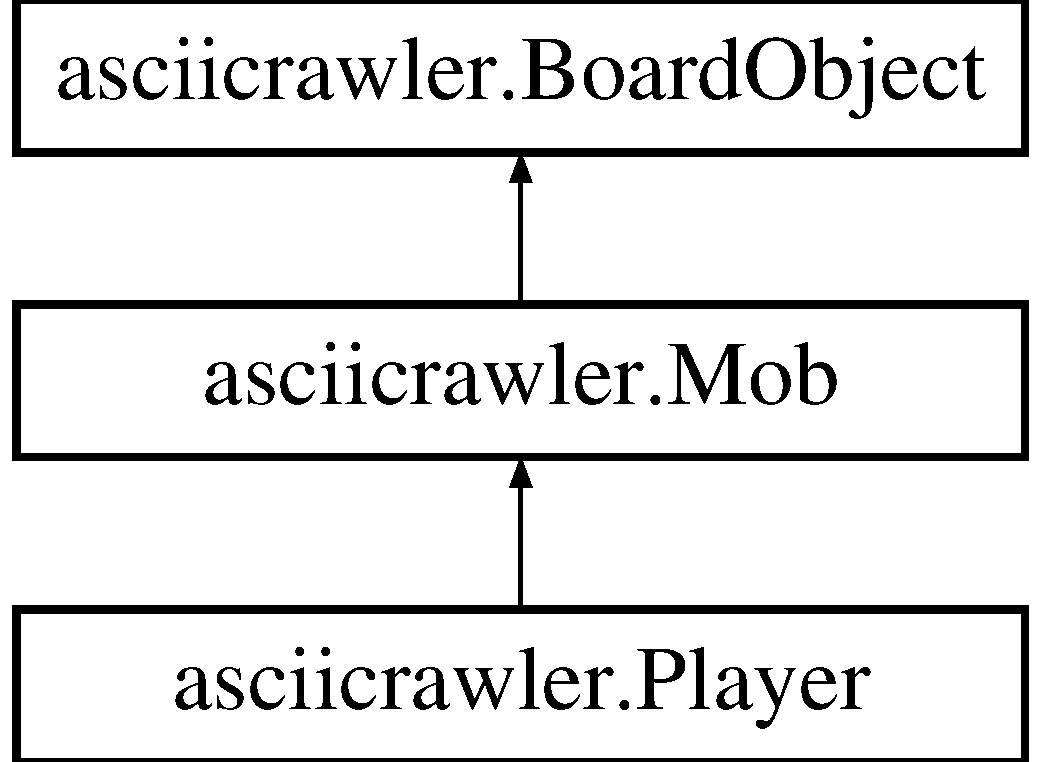
\includegraphics[height=3.000000cm]{classasciicrawler_1_1Player}
\end{center}
\end{figure}
\subsection*{Public Member Functions}
\begin{DoxyCompactItemize}
\item 
Color \hyperlink{classasciicrawler_1_1Player_a5c51590842281f692f09826886933be7}{get\+Color} ()
\item 
boolean \hyperlink{classasciicrawler_1_1Player_a45d5a582e0d18c69ac72b19218b00a97}{can\+Enter} ()
\item 
void \hyperlink{classasciicrawler_1_1Player_af176593345048bd28121f41f7e6d1723}{move} ()
\end{DoxyCompactItemize}
\subsection*{Additional Inherited Members}


\subsection{Detailed Description}
\hyperlink{classasciicrawler_1_1Player}{Player} is class derived from mob. It specifices the abilities and and actions of a player. 

\begin{DoxyAuthor}{Author}
Leon Hansen, Felix Schmidt 
\end{DoxyAuthor}
\begin{DoxyVersion}{Version}
1.\+0 
\end{DoxyVersion}


\subsection{Member Function Documentation}
\mbox{\Hypertarget{classasciicrawler_1_1Player_a45d5a582e0d18c69ac72b19218b00a97}\label{classasciicrawler_1_1Player_a45d5a582e0d18c69ac72b19218b00a97}} 
\index{asciicrawler\+::\+Player@{asciicrawler\+::\+Player}!can\+Enter@{can\+Enter}}
\index{can\+Enter@{can\+Enter}!asciicrawler\+::\+Player@{asciicrawler\+::\+Player}}
\subsubsection{\texorpdfstring{can\+Enter()}{canEnter()}}
{\footnotesize\ttfamily boolean asciicrawler.\+Player.\+can\+Enter (\begin{DoxyParamCaption}{ }\end{DoxyParamCaption})\hspace{0.3cm}{\ttfamily [inline]}}

set that the enemies can enter a player \mbox{\Hypertarget{classasciicrawler_1_1Player_a5c51590842281f692f09826886933be7}\label{classasciicrawler_1_1Player_a5c51590842281f692f09826886933be7}} 
\index{asciicrawler\+::\+Player@{asciicrawler\+::\+Player}!get\+Color@{get\+Color}}
\index{get\+Color@{get\+Color}!asciicrawler\+::\+Player@{asciicrawler\+::\+Player}}
\subsubsection{\texorpdfstring{get\+Color()}{getColor()}}
{\footnotesize\ttfamily Color asciicrawler.\+Player.\+get\+Color (\begin{DoxyParamCaption}{ }\end{DoxyParamCaption})\hspace{0.3cm}{\ttfamily [inline]}}

returns the color of the player \mbox{\Hypertarget{classasciicrawler_1_1Player_af176593345048bd28121f41f7e6d1723}\label{classasciicrawler_1_1Player_af176593345048bd28121f41f7e6d1723}} 
\index{asciicrawler\+::\+Player@{asciicrawler\+::\+Player}!move@{move}}
\index{move@{move}!asciicrawler\+::\+Player@{asciicrawler\+::\+Player}}
\subsubsection{\texorpdfstring{move()}{move()}}
{\footnotesize\ttfamily void asciicrawler.\+Player.\+move (\begin{DoxyParamCaption}{ }\end{DoxyParamCaption})\hspace{0.3cm}{\ttfamily [inline]}}

defines the movements of the player on a specific key event 

The documentation for this class was generated from the following file\+:\begin{DoxyCompactItemize}
\item 
/home/felix/\+Documents/\+Uni/\+Master/1. Semester/\+Technische Dokumentation/\+Spiel/\+Ascii-\/\+Crawler/src/asciicrawler/Player.\+java\end{DoxyCompactItemize}

\hypertarget{classasciicrawler_1_1Wall}{}\section{asciicrawler.\+Wall Class Reference}
\label{classasciicrawler_1_1Wall}\index{asciicrawler.\+Wall@{asciicrawler.\+Wall}}


\hyperlink{classasciicrawler_1_1Wall}{Wall} is a board object. This field can not entered by any mob.  


Inheritance diagram for asciicrawler.\+Wall\+:\begin{figure}[H]
\begin{center}
\leavevmode
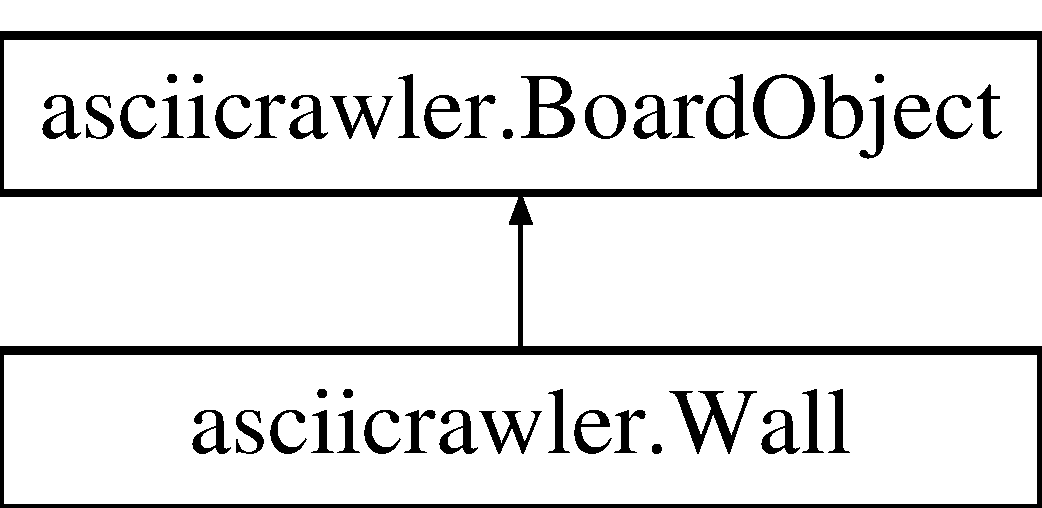
\includegraphics[height=2.000000cm]{classasciicrawler_1_1Wall}
\end{center}
\end{figure}
\subsection*{Public Member Functions}
\begin{DoxyCompactItemize}
\item 
boolean \hyperlink{classasciicrawler_1_1Wall_a02f8695f9861d61b9d2c3af3a185e522}{can\+Enter} ()
\item 
Color \hyperlink{classasciicrawler_1_1Wall_a357f77acaa033e6d59b5973459954bb8}{get\+Color} ()
\end{DoxyCompactItemize}


\subsection{Detailed Description}
\hyperlink{classasciicrawler_1_1Wall}{Wall} is a board object. This field can not entered by any mob. 

\begin{DoxyAuthor}{Author}
Leon Hansen, Felix Schmidt 
\end{DoxyAuthor}
\begin{DoxyVersion}{Version}
1.\+0 
\end{DoxyVersion}


\subsection{Member Function Documentation}
\mbox{\Hypertarget{classasciicrawler_1_1Wall_a02f8695f9861d61b9d2c3af3a185e522}\label{classasciicrawler_1_1Wall_a02f8695f9861d61b9d2c3af3a185e522}} 
\index{asciicrawler\+::\+Wall@{asciicrawler\+::\+Wall}!can\+Enter@{can\+Enter}}
\index{can\+Enter@{can\+Enter}!asciicrawler\+::\+Wall@{asciicrawler\+::\+Wall}}
\subsubsection{\texorpdfstring{can\+Enter()}{canEnter()}}
{\footnotesize\ttfamily boolean asciicrawler.\+Wall.\+can\+Enter (\begin{DoxyParamCaption}{ }\end{DoxyParamCaption})\hspace{0.3cm}{\ttfamily [inline]}}

Checks if the \hyperlink{classasciicrawler_1_1Mob}{Mob} can access this type of field \mbox{\Hypertarget{classasciicrawler_1_1Wall_a357f77acaa033e6d59b5973459954bb8}\label{classasciicrawler_1_1Wall_a357f77acaa033e6d59b5973459954bb8}} 
\index{asciicrawler\+::\+Wall@{asciicrawler\+::\+Wall}!get\+Color@{get\+Color}}
\index{get\+Color@{get\+Color}!asciicrawler\+::\+Wall@{asciicrawler\+::\+Wall}}
\subsubsection{\texorpdfstring{get\+Color()}{getColor()}}
{\footnotesize\ttfamily Color asciicrawler.\+Wall.\+get\+Color (\begin{DoxyParamCaption}{ }\end{DoxyParamCaption})\hspace{0.3cm}{\ttfamily [inline]}}

Returns the Color of the field 

The documentation for this class was generated from the following file\+:\begin{DoxyCompactItemize}
\item 
/home/felix/\+Documents/\+Uni/\+Master/1. Semester/\+Technische Dokumentation/\+Spiel/\+Ascii-\/\+Crawler/src/asciicrawler/Wall.\+java\end{DoxyCompactItemize}

\hypertarget{classasciicrawler_1_1Water}{}\section{asciicrawler.\+Water Class Reference}
\label{classasciicrawler_1_1Water}\index{asciicrawler.\+Water@{asciicrawler.\+Water}}


\hyperlink{classasciicrawler_1_1Water}{Water} is a board object. This field can not entered by any mob.  


Inheritance diagram for asciicrawler.\+Water\+:\begin{figure}[H]
\begin{center}
\leavevmode
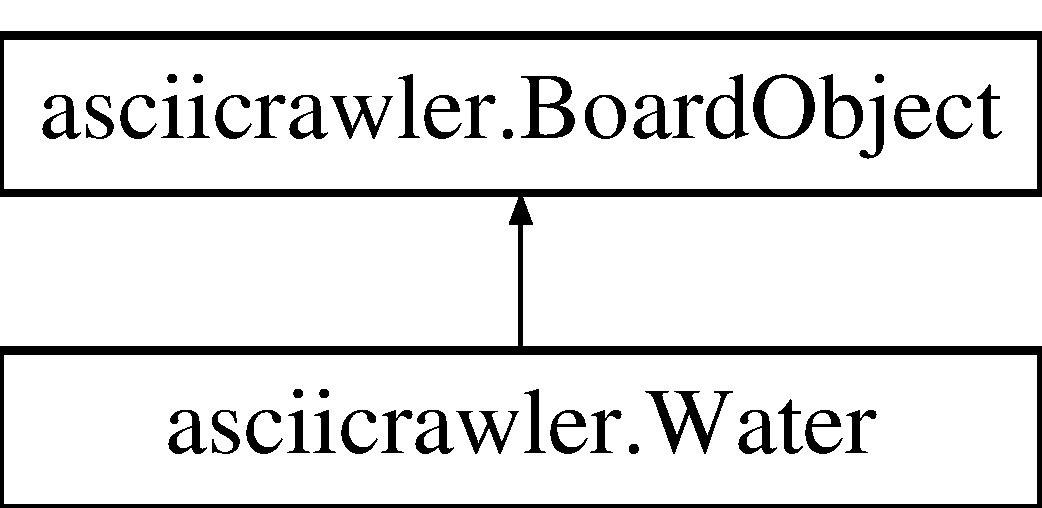
\includegraphics[height=2.000000cm]{classasciicrawler_1_1Water}
\end{center}
\end{figure}
\subsection*{Public Member Functions}
\begin{DoxyCompactItemize}
\item 
boolean \hyperlink{classasciicrawler_1_1Water_a181a9e47757f74bc49d4df4f8a6677ab}{can\+Enter} ()
\item 
Color \hyperlink{classasciicrawler_1_1Water_a43367f040a73539cdd92421cc351b4ca}{get\+Color} ()
\end{DoxyCompactItemize}


\subsection{Detailed Description}
\hyperlink{classasciicrawler_1_1Water}{Water} is a board object. This field can not entered by any mob. 

\begin{DoxyAuthor}{Author}
Leon Hansen, Felix Schmidt 
\end{DoxyAuthor}
\begin{DoxyVersion}{Version}
1.\+0 
\end{DoxyVersion}


\subsection{Member Function Documentation}
\mbox{\Hypertarget{classasciicrawler_1_1Water_a181a9e47757f74bc49d4df4f8a6677ab}\label{classasciicrawler_1_1Water_a181a9e47757f74bc49d4df4f8a6677ab}} 
\index{asciicrawler\+::\+Water@{asciicrawler\+::\+Water}!can\+Enter@{can\+Enter}}
\index{can\+Enter@{can\+Enter}!asciicrawler\+::\+Water@{asciicrawler\+::\+Water}}
\subsubsection{\texorpdfstring{can\+Enter()}{canEnter()}}
{\footnotesize\ttfamily boolean asciicrawler.\+Water.\+can\+Enter (\begin{DoxyParamCaption}{ }\end{DoxyParamCaption})\hspace{0.3cm}{\ttfamily [inline]}}

Checks if the \hyperlink{classasciicrawler_1_1Mob}{Mob} can access this type of field \mbox{\Hypertarget{classasciicrawler_1_1Water_a43367f040a73539cdd92421cc351b4ca}\label{classasciicrawler_1_1Water_a43367f040a73539cdd92421cc351b4ca}} 
\index{asciicrawler\+::\+Water@{asciicrawler\+::\+Water}!get\+Color@{get\+Color}}
\index{get\+Color@{get\+Color}!asciicrawler\+::\+Water@{asciicrawler\+::\+Water}}
\subsubsection{\texorpdfstring{get\+Color()}{getColor()}}
{\footnotesize\ttfamily Color asciicrawler.\+Water.\+get\+Color (\begin{DoxyParamCaption}{ }\end{DoxyParamCaption})\hspace{0.3cm}{\ttfamily [inline]}}

Returns the Color of the field 

The documentation for this class was generated from the following file\+:\begin{DoxyCompactItemize}
\item 
/home/felix/\+Documents/\+Uni/\+Master/1. Semester/\+Technische Dokumentation/\+Spiel/\+Ascii-\/\+Crawler/src/asciicrawler/Water.\+java\end{DoxyCompactItemize}

%--- End generated contents ---

% Index
\backmatter
\newpage
\phantomsection
\clearemptydoublepage
\addcontentsline{toc}{chapter}{Index}
\printindex

\end{document}
